\documentclass[12pt,letterpaper]{article}
\usepackage[DIV=14,BCOR=2mm,headinclude=true,footinclude=false]{typearea}

%\usepackage[urw-garamond]
%\usepackage[T1]{fontenc}

\renewcommand{\baselinestretch}{1.15} 
\usepackage[affil-it]{authblk}
\usepackage{latexsym}
\usepackage{amsmath}
\usepackage{MinionPro}
\usepackage{hyperref}
\usepackage{tikz}
\usepackage{verbatim}
\usepackage{natbib}
\usepackage{color, colortbl}
\usepackage{appendix}
\usepackage{amsmath,amsthm}


%\usepackage{wasysym}
%\usepackage{amssymb}

\usetikzlibrary{arrows,shapes}

\definecolor{Gray}{gray}{0.9}

\newtheorem{result}{Result}
\newtheorem*{main result}{Main Result}
\newtheorem{theorem}{Theorem}
\newtheorem{conjecture}{Conjecture}[section]
\newtheorem{corollary}{Corollary}[section]
\newtheorem{lemma}{Lemma}[section]
\newtheorem{proposition}{Proposition}[section]
\newtheorem{definition}{Definition}[section]
\newtheorem{assumption}{Assumption}[section]


\theoremstyle{definition}
\newtheorem{example}{Example}[section]

\theoremstyle{remark}
\newtheorem*{remark}{Remark}

\theoremstyle{claim}
\newtheorem{claim}{Claim}


\pgfdeclarelayer{background}
\pgfsetlayers{background,main}

\tikzstyle{vertex}=[circle,fill=black!25,minimum size=12pt,inner sep=0pt]
\tikzstyle{selected vertex} = [vertex, fill=red!24]
\tikzstyle{edge} = [draw,thick,-]
\tikzstyle{weight} = [font=\small]
\tikzstyle{selected edge} = [draw,line width=5pt,-,red!50]
\tikzstyle{ignored edge} = [draw,line width=5pt,-,black!20]


\linespread{1.2}

\begin{document}
%\fontsize{12}{20pt}\selectfont



\title {Coordination in Social Networks : Communication by Actions}


\author {Chun-Ting Chen\thanks{cuc230@psu.edu. I would like to thank Kalyan Chatterjee for his guidance, encouragement, and tremendous support. I am also indebted to Edward Green, James Jordan and Neil Wallace for their substantial advice and guidance. I would like also to thank Yu Awaya, Mohammad Davoodalhoseini, Chen-Ying Huang, Vijay Krishna, and Nozawa Wataru for their helpful comments and suggestions. All remaining errors are my own.}}
\affil{The Pennsylvania State University}

%\date{December 12, 2014}



\maketitle








\begin{abstract}

This paper studies a collective action problem in a setting of discounted repeated coordination games where information and monitoring structures are modeled as networks. Players only know their neighbors' types that describe the neighbors' inclination to participate in a collective action as well as monitor their neighbor's past actions. I ask what kinds of networks can induce people to solve the uncertainty about players' inclination and coordinate to the ex-post efficient outcome.

In order to coordinate to the ex-post efficient outcome, players need to communicate by their actions and there should be ``routes'' for players to communicate. I define strong connectedness to characterize such routes. A state has strong connectedness if and only if for every two players who incline to participate, there is a path consisting of players who have the same types to connect them. Given that the networks are fixed, finite, connected, commonly known, and undirected, if such networks are without cycles, I show that, for all priors with full support on the strong connectedness states, there is a (weak) sequential equilibrium path in which the ex-post efficient outcome repeats after a finite time $T$ when discount factor is sufficiently high. Given that the states of nature are discrete, this equilibrium is constructive and does not depend on public or private signals other than players' actions.



\end{abstract}








\section{Introduction} 

This paper studies collective action in a setting of discounted repeated coordination games, in which information and monitoring structures are modeled as networks. Players are uncertain about the state of nature but can observe their neighbors' actions. I ask what kind of networks can induce players to solve the underlying uncertainty in order to coordinate to the ex-post efficient outcome. Although the main motivation is to understand the dynamics of social movement, I focus on the collective action within social structures.

Strong discontent exists with the goal to overthrow an authoritarian regime. However, it may be difficult to organize movements because knowledge about the existence of such discontents is not always transparent. For instance, the East Germany government had control over the electoral system and the mass media. The secret agents also deterred individuals from showing their discontent. As \citep{Karl-Dieter1993} and \citep{Chwe2000} suggest, discontent may be revealed ``locally'' through individuals' personal networks but difficult to diffuse to the general public. As strong discontent is often private, the lack of knowledge of the general consensus may prevent people from conducting a one-shot uprising when faced with consequences of failure in an autocracy. \citep{Chwe2000} characterizes the networks that provide common knowledge about peoples' discontent by investigating a one-shot incomplete information collective action in networks. On the other hand, \citep{Lohmann2011} considers multi-periods collective action and uses informational cascade model to explain events that trigger following actions, such as the consecutive demonstrations in East Germany during 1989-1991. When rebels are aware of their capacity in transmitting relevant information about the level of collective discontent, they may be willing to act although risks still exist. I view the acts to take the risks in participating in collective action a part of an equilibrium strategy, making the entire movement a learning process.


Inspired by \citep{Chwe2000}, I model such dynamic collective action in the following way. Players repeatedly play a $k$-\textit{Threshold game} with a parameter $k$ in a network. Two types of players are present in the network: \textit{Rebel} and \textit{Inert}.  Players' types and their actions can be observed only by their neighbors. A Rebel can take two kinds of actions: \textbf{revolt} and \textbf{stay}. An Inert can only \textbf{stay}. A Rebel will get pay-off as $1$ if he chooses \textbf{revolt} and more than $k$ players choose \textbf{revolt}; he will get pay-off as $-1$ if he chooses \textbf{revolt} and less than $k$ players choose \textbf{revolt}; he will get pay-off as $0$ if he chooses \textbf{stay}. An Inert will get pay-off as $1$ if he chooses \textbf{stay}.

Since a Rebel may not know how many Rebels are present, Rebels' pay-off structure captures the idea that \textbf{stay} is a safe action and \textbf{revolt} is a risky action. Given a common prior $\pi$ over players' types, players play this $k$-Threshold game infinitely repeatedly with a common discount factor $\delta$. Cheap talk is not allowed; no outside mechanism can serve as an information exchange device. 


Rebels then communicate with each other by their actions. For different $k$ and different network structures, I look for a sequential equilibrium which has the property of \textit{approaching ex-post efficient} (\textit{APEX} henceforth) to investigate the information-sharing behavior in the networks. An equilibrium is APEX if and only if \textit{the tails of actions in the equilibrium path repeats the static ex-post efficient outcome after a finite time $T$}. This refinement confirms if players learns the relevant information in finite time. If there are at least $k$ Rebels in this society, then all Rebels should \textbf{revolt} after $T$ as if they are certain that more than $k$ Rebels exist; otherwise, all Rebels should \textbf{stay} after $T$. Rebels' incentives to communicate are affected by Rebels' positions in networks since information and monitoring are constructed through networks.

In order to achieve a quick intuition about Rebels' learning process in the proposed framework, we may consider the $k$-Threshold game with $k=n$ and assume that pay-off is hidden. When $k=n$, a Rebel can get positive pay-off only if all the players are Rebels. Given that the networks are fixed, finite, connected, commonly known, and undirected (\textit{FFCCU} henceforth), an APEX sequential equilibrium can be constructed and explained by a contagion-like argument. This argument is to treat \textbf{stay} as a message that ``there is an Inert out there'' and treat revolt as a message that ``there could be no Inert out there''. If a Rebel has an Inert neighbor, then he plays \textbf{stay} forever. If he has no Inert neighbors, then he plays \textbf{revolt} until he observes that some of his neighbors play \textbf{stay}, and then he shifts to play \textbf{stay} forever. Since the networks are FFCCU, within finite periods, a Rebel will learn that there is an Inert out there if some neighbors has played \textbf{stay} and will learn that there is no an Inert out there otherwise.


The non-trivial cases appear when $k<n$. The $k=n$ case is easier because the underlying relevant information is to indicate if ``there is an Inert out there.'' I construct equilibrium when $k=n$ by using single-period binary actions, $\{\textbf{stay},\textbf{revolt}\}$ to separate the states into two parts: ``no Inerts'' or ``some Inerts''. In other words, these single-period actions can generate distinguishable signals to inform players by telling the true states of nature\footnote{e.g., \citep{Fudenberg2010} or \citep{Fudenberg2011}.}. However, when $k<n$, the relevant information is to answer ``Are there at least k Rebels out there? '', and these binary actions serve to reveal such relevant information. As I will show later, several sequences of actions will be used to transmit Rebels' private information and to control Rebels' beliefs in the equilibrium. In the equilibrium path, two kinds of sequence will be used. \textit{Reporting messages} reports their private information about the state of nature. \textit{Coordination messages} informs Rebels about whether some other Rebels possess the relevant information. Specifically, in the equilibrium path, Rebels will send the coordination message to inform nearby Rebels whenever they learn relevant information. Those nearby Rebels will play the same message again to inform their nearby Rebels. The coordination message serves as a short-cut to track individuals' higher-order beliefs about ``Do any Rebels have the relevant information? '', ``Do any Rebels know that some Rebels have the relevant information?'', etc.



It is important to note that communication is costly in the sense that playing revolt is risky. Due to being discounting, Rebels always seek the opportunity to manipulate their messages to save cost in the time horizontal line \footnote{Indeed, allowing cheap talk or using limit-of-mean preference (e.g., \citep{Renault1998}) will solve this coordination problem.}. A free rider problem may occur when reporting information incurs costs. I give an example here to illustrate this issue\footnote{Example ~\ref{ex_free_rider_tree}}. In a situation where two nearby Rebels exchange information  , let's suppose that these two Rebels can learn the true state after acquiring information from each other's truthful reporting. Let's further suppose that each of them can freely initiate coordination after exchanging information. In this instance, truthful reporting is not a best response because a player can wait given that the other will report truthfully. The above scenario demonstrates future coordination as a public good. This public good can only be made by Rebels' truthful reporting, which incurs costs.


The main result will show that this coordination problem can be solved in the FFCCU networks \textit{without cycles}. Here, I define an (acyclic) \textit{path} in $G$ as a sequence consisting of nodes without repetition in which a succeeding node is a neighbor of the previous node. I also define an undirected network $G$ without cycles by defining a network in which the path between different nodes is unique. After I define \textit{strong connectedness} as the property in which a path consisting of Rebels exists to connect any pairs of Rebels. The main result shows:



\begin{main result}
In any FFCCU network without cycles, if $\pi$ has full support on the strong connectedness, then for $n$-person repeated $k$-Threshold game with parameter $1\leq k \leq n$, there is a $\delta^{*}$ such that a (weak) APEX sequential equilibrium exists whenever $\delta\in (\delta^{*},1)$.  
\end{main result}

Here, $\pi$ has full support on strong connectedness, which means that $\pi$ assigns positive probability on the states that have strong connectedness and only assigns positive probability on those states. This assumption is to ensure that the underlying game is not reduced to an incomplete information game without communication. To see this, we may recall that an Inert always plays \textbf{stay}. Rebels can not communicate with any Rebels through their actions if an Inert happens to separate them. For instance, in a wheel network, an incomplete game without communication is that the central player is an Inert while the peripheral players are all Rebels. It is impossible to find an APEX equilibrium in this instance unless $k=1$.



The off-path belief serves as a grim trigger as follows. Whenever a Rebel detects a deviation, he believes that all other players outside his neighborhood are Inerts. Thus, if there are less than $k$ Rebels in his neighborhood, he will play \textbf{stay} forever. With this off-path belief and the constructed equilibrium strategies, the belief system satisfies \textit{updating consistency}(\citep{Perea2002}), while it may not satisfies full consistency (\citep{Krep_Wilson1982}). \footnote{ Updating consistency requires that, for every player, for every player's strategies, for every information sets $s^1,s^2$ where $s^2$ follows $s^1$, if $s^2$ happens with positive probability given $s^1$ and given players' strategies contingent on $s^1$, then the belief over $s^2$ should satisfy Bayesian updating conditional on the belief over $s^1$ and players' strategies contingent on $s^1$. In other words, the updating consistency require that players hold beliefs in every information sets and hold updating beliefs that follows previous beliefs. This requirement imposes restrictions on off-path beliefs that induce sequential rationality, although it is weaker than full consistency in the sense that full consistency implies updating consistency.}

The equilibrium construction starts from building a communication protocol. By exploiting the assumption of finite and commonly known network, I assign each node a distinct prime number. Then I construct reporting messages and let them to carry information about the multiplication of nodes' prime numbers. Since the multiplication of prime numbers can be de-factorized uniquely, the reporting messages thus carry the information about those nodes' locations in a network. Next, I let two phases, \textit{reporting period} and \textit{coordination period}, alternate in the time horizon, where the reporting (resp. coordination) messages are played in the reporting (resp. coordination) period. In coordination period, whenever a Rebel can tell the relevant information, such Rebel inform his nearby Rebels by sending coordination messages. Those nearby Rebels then continue to inform their nearby Rebels by sending coordination messages, etc. By exploiting the assumption of FFCCU network, after coordination period Rebels have commonly known that all Rebels can tell the relevant information if they have received coordination messages.

I call a complete two-phases, starting from a reporting period and ending with a following coordination period, a \textit{block}. In a block, I control the inter-temporal incentives in playing between reporting and coordination messages as follows. First, I let both of the coordination messages, one of them can initiate the coordination to \textbf{revolt} and another one can initiate the coordination to \textbf{stay}, incur no expected cost. Second, I let Rebels play \textbf{revolt} after a block only if they have observed the coordination message to \textbf{revolt} and observed some reporting messages which incur expected cost. I let, however, the continued behavior after observing the coordination message to \textbf{stay} is not contingent on any reporting message. When a Rebel sees potential future coordination to \textbf{revolt}, he may have an incentive to ``spend money'' to influence Rebels' future behavior forwardly; otherwise, he just plays stay. Next, in the equilibrium path, I make sure that Rebels plays ex-post efficient outcome repeatedly right after a block if some Rebels initiate the coordination in that block. I argue that only those Rebels who learn relevant information after reporting period have the incentive to initiate coordination since they do not need further information to tell the state. This argument shows that a Rebel other than them will not take advantage to send that free coordination message to initiate coordination. This is because players can not update further information if all of their neighbors continue to play the same actions in the future. When $\delta$ is high enough, he will not initiate coordination which may impede his own learning process to achieve the ex-post efficient outcome.

I then characterize Rebels' incentive in spending money and control how much money they should spend to sustain an APEX equilibrium. In the equilibrium path, a Rebel iteratively updates his relevant information given other Rebels' money-spending in reporting their information about the state, and a Rebel spends moneys only if his current relevant information has not been acquired by other Rebels. In the equilibrium path, a Rebel thus believes that ``more other Rebels are out there'' if and only if his nearby Rebel spends money to report their existence. Some specified forms of reporting messages are introduced, and the off-path belief enforces Rebels not to play differently from them.

The key step here is to construct a reporting message, ``spend a money'', which incurs the least expected cost; this message should be considered as a part of equilibrium path. I denote this special money as $\langle 1 \rangle$. To see its importance, I consider the concept of ``pivotal Rebel''. Here, a pivotal Rebel is the Rebel who attains relevant information immediately after a reporting period ends under the condition that other Rebels report their information truthfully before the pivotal Rebel spends money. Now I suppose playing $\langle 1 \rangle$ is not a part of equilibrium path, and suppose a Rebel find that he himself is a pivotal Rebel during a reporting period without having reported anything during that period. He may then find a profitable deviation by spending less money, which can not be detected by at least k Rebels although some Rebels can detect such deviation. Since those Rebels who detect such deviation will play \textbf{stay} forever by the off-path belief, and this pivotal Rebel can initiate coordination to \textbf{revolt} by convincing other Rebels to play \textbf{revolt}, the APEX fails. To solve this problem, I introduce message $\langle 1 \rangle$ to let pivotal Rebels identify themselves, while coordination messages to \textbf{revolt} or to \textbf{stay} have to be initiated immediately after $\langle 1 \rangle$ has been played in the equilibrium path.

Under the circumstances in which multiple pivotal players are nearby one another, the APEX may fail because playing $\langle 1 \rangle$ does not explicitly address the number of Rebels learned by pivotal players. The assumption of acyclic networks is crucial to solving these problems. If the networks are acyclic, I will show later that there are only two kinds of pivotal Rebels. One kind is that they recognize that there are at least $k-1$ Rebels. The other kind is that they will know the true state based on other Rebels' truthful reporting. The latter might become a free rider problem because they may not recognize that there are at least $k-1$ Rebels.  If the networks are acyclic, Lemma ~\ref{lemma_at_most_two_nodes} will show that the free rider problem only occurs between the two nearby pivotal Rebels in only one block in the equilibrium path. Further, these two nearby Rebels will know that this free rider problem will occur before entering this block. Depending on their indexed prime numbers, one of them reports about the state, and the other one plays $\langle 1 \rangle$ in the equilibrium. 






This paper contributes to several fields of economics. 


First, future coordination can be viewed as a public good among all Rebels. A strand of public good literature, such as \citep{Lohmann1994}, views information as a public good while generating information is also costly \footnote{For instance, \citep{Lohmann1993}\citep{Lohmann1994} consider that individuals generate information by their actions, where the aggregate outcomes of actions is public. \citep{Bolto_Harris1999} consider team experiment in infinite time horizon where the outcomes of experiments are public signals. \citep{Bramoulle2007} view information as a public good and consider public good provision in networks.}. This paper models costly information generation and adds another aspect--- network-monitoring--- to investigate collective action.


Second, this paper is related to the literature in social learning \footnote{Reviews can be seen in \citep{Bikhchandani1998} \citep{Cao2001}.} . Several papers have considered social learning in networks\footnote{\citep{Goyal2012} gives the reviews. Recent papers, e.g., \citep{Acemoglu2011}\citep{Chatterjee2011}, also discuss this topic} . In this literature, when players are myopic, the information flow could be very complicated because the information they send can affect their future behavior. For instance, in \citep{RePEc:eee:gamebe:v:45:y:2003:i:2:p:329-346}, even for 3-person undirected networks, the complete and incomplete networks will give different results depending on individuals' initial private signals and allocations in a network. Instead of using Bayesian learning, \citep{Golub2010} use a naive learning protocol to tackle this social learning problem. I consider social learning in networks as a learning-in-game procedure, where an individual may put more weight on the future learning results. My result suggests that the shape of the network (without cycle) is not significant if players are far-sighted.

Third, a growing body of literature studies the game played in networks where various games played in different networks with varying definitions \footnote{\citep{Jackson2008}\citep{Goyal2012} gives the reviews.}. Only few papers discuss the repeated game. In complete information game, Laclau2012 proves a folk theorem where players play the game locally. \citep{Wolitzky2013} \citep{Wolitzky2014} consider network-like monitoring where a prisoner dilemma game is played globally. My paper is the first paper to consider the incomplete information game repeatedly played in a network. 


My paper is also related to folk theorems in discounted repeated game with incomplete information. In this literature, they consider more general games than the games adopted here. \citep{Fudenberg2010} \citep{Fudenberg2011} \citep{Wiseman2012}  considering $n$-person game with public signals jointly generated by the states and actions; \citep{Yamamoto2014} consider $2$-person game with private signals jointly generated by the states and actions. The full-rank conditions are imposed to allow single-period actions to generate informative signals to separates the states. Here, I consider $n$-person game without signals and thus do not impose the single-period full-rank conditions before solving the equilibrium. I do not mean to prove a folk theorem here. My results, however, show that the FFCCU networks without cycles suffice in approaching the ex-post efficiency when discount factor is high enough.


The paper is organized as the followings. Section ~\ref{sec:model} introduces the model. Section ~\ref{sec:equilibrium} discusses the equilibrium construction and shows the main result. Some variations of my model will be discussed in its subsection ~\ref{sec:varies}. Section ~\ref{sec:con} makes the conclusion. All the missing proofs can be found in the Appendix.

\section{Model}
\label{sec:model}
\subsection{Notations}
Given a finite set $A$, let $\#A$ denote the cardinality of a set $A$, and let $\Delta A$ denote the set of probability distributions over $A$. 

The square bracket $[]$ following a quantifier, $\exists$ or $\forall$, will be read as ``\textit{such that}''. For instance, $\exists a \in A [c\in A, c=a]$ will be read as ``exists $a$ in $A$ such that $c$ is in A and $c$ is equal to $a$.'' .
\subsection{Model}


There are $n$ players. $N=\{1,2,...,n\}$ denotes the set of players.  Let $G$ be a network if  $G$ is a point-to-set function mapping from $N$ to a subset of $N$ containing $i\in N$. Moreover,  let $G_i=G(i)$ be $i$'s neighbors and also let $\bar{G}_i=G_i\backslash \{i\}$ be $i$'s neighborhood excluding $i$ itself. $G$ is fixed if $G$ is not random, and $G$ is undirected if for all $i,j$ if $j\in G_i$ then $i\in G_j$. Throughout this paper, I assume $G$ is finite, fixed, commonly known, and undirected. 

For each player $i$, let $\Theta_i=\{Rebel,Inert\}$ and let $\theta_i\in \Theta_i$ denotes an element in $\Theta_i$. I call $\theta_i$ as player $i$'s ``type''. The set of states of nature is $\Theta=\prod_{j\in N}\Theta_j$ and let $\theta\in \Theta$ be a state of nature. For convenience, let $[Rebels](\theta)=\{j:\theta_j=Rebel\}$ be the set of Rebels given $\theta$, and let $\Theta_{G_i}=\prod_{j\in G_i}\Theta_j$ and $\theta_{G_i}\in \Theta_{G_i}$. Let $p_{G_i}:\Theta \rightarrow 2^{\Theta}$ be $i$'s information partition function such that $p_{G_i}(\theta)=\{\theta_{G_i}\}\times \prod_{j\not\in G_i}\Theta_j$, and let $\mathcal{P}_{G_i}=\{p_{G_i}(\theta)\}_{\theta\in \Theta}$ be $i$'s information sets about $\theta$. In other words, whenever nature chooses a state, $i$ knows his own $\theta_i$ and his neighbor $j$'s $\theta_j$. 

There is a game, $k$-threshold game, played infinitely repeatedly  with a common discounted factor $\delta$ in a fixed $G$. Time is discrete. At the beginning of this game, a state is realized and there is a common prior $\pi\in \Delta \Theta$ over $\Theta$. After a state is realized, that state is fixed over time, and players simultaneously choose an action $a_{\theta_i}\in A_{\theta_i}$ in each period afterwards. If $\theta_i=Rebel$, then $A_{\theta_i}=\{\textbf{revolt}, \textbf{stay}\}$.  If $\theta_i=Inert$, then $A_{\theta_i}=\{\textbf{stay}\}$. Let $a_{\theta_i}\in A_{\theta_i}$ be $i$'s action if $i$'s type is $\theta_i$, and let $a_{-\theta_i}\in \Pi_{j\in N,j\neq i}A_{\theta_j}$ be the actions taken by players other than $i$. Player $i$'s stage pay-off function, $u_{\theta_i}: \Pi_{j\in N}A_{\theta_j}\rightarrow \mathbb{R}$, is defined as follows. 
\begin{enumerate}
\item $u_{Rebel_i}(a_{Rebel_i},a_{-\theta_i})=1$ if $a_{Rebel_i}=\textbf{revolt}$ and $\#\{j:a_{\theta_j}=\textbf{revolt}\}\geq k$
\item $u_{Rebel_i}(a_{Rebel_i},a_{-\theta_i})=-1$ if $a_{Rebel_i}=\textbf{revolt}$ and $\#\{j:a_{\theta_j}=\textbf{revolt}\}< k$
\item $u_{Rebel_i}(a_{Rebel_i},a_{-\theta_i})=0$ if $a_{Rebel_i}=\textbf{stay}$
\item $u_{Inert_i}(a_{Inert_i},a_{-\theta_i})=1$ if $a_{Inert_i}=\textbf{stay}$
\end{enumerate}

Players can observe their neighbors' actions perfectly but cannot observe others' actions. For simplicity, I assume that pay-off is hidden until Section \ref{sec:varies}. Let $s\geq 0$ denote a period. Define $H^0_{i}=\{ \emptyset \}$ and define $H^s_{i}=H^0_{i}\times \prod^s_{t=1}A_{\theta_i}$ to be the set of histories of actions played by player $i$ up to period $s$. Define $H^0_{G_i}=\{\emptyset\}$ and define $H^s_{G_i}=H^0_{G_i}\times \prod^s_{t=1}\prod_{j\in G_i}A_{\theta_j}$ to be the set of histories player $i$ can observe up to period $s$.  For convenience, also define $H^0=\{\emptyset\}$, $H^s=H^0\times \prod^s_{t=1}\prod_{j\in N}A_{\theta_j}$, and $H=H^0\times \prod^{\infty}_{s=1}\prod_{j\in N}A_{\theta_j}$ with generic element $h\in H$. Up to period $s$, $i$'s information sets related to histories of actions are $\mathcal{H}^s_{G_i}=\{\{h^s_{G_i}\}\times \prod_{j\notin G_i}H^s_{j}\}_{h^s\in H^s}$, where $h^s_{G_i}\in H^s_{G_i}$.

$i$'s pure strategy is defined by $\tau_{\theta_i}:(\prod_{j\in G_i}\Theta_j)\times \bigcup^{\infty}_{s=0}H^s_{G_i}\rightarrow A_{\theta_i}$. For convenience, also define $\tau=\{\tau_{\theta_i}\}_i$. 
 
The prior $\pi$, the network $G$, and the strategy $\tau$ jointly induce a distribution, $\gamma^{\pi,\tau}_G$, over $\Theta\times H$. Given a realization $(\theta,h)$ according to $\gamma^{\pi,\tau}_G$, let $h^{\tau}_\theta$ be the realized sequence of actions generated by $\tau$ given $\theta$. 
For each player $i$,  for each period $s$, $\alpha^{\pi,\tau}_{G_i}(\theta, h^{s}|\theta_{G_i},h^{s}_{G_i})$ denotes the conditional distribution over $\Theta\times H^s$ induced by $\tau$ and conditional on $(\theta_{G_i}, h^{s}_{G_i} )$, where $\theta_{G_i}\in \Theta_{G_i}$ and $h^{s}_{G_i}\in H^s_{G_i}$. For convenience, also define $\beta^{\pi,\tau}_{G_i}(\theta|\theta_{G_i},h^{s}_{G_i})=\sum_{h^{s}\in H^s}\alpha^{\pi,\tau}_{G_i}(\theta, h^{s}|\theta_{G_i},h^{s}_{G_i})$.
Finally, let
$E^{\delta}_G(u_{\theta_i}(\tau)|\alpha^{\pi,\tau}_{G_i}(\theta, h^{s}|\theta_{G_i},h^{s}_{G_i}))$
be $i$'s continuation expected pay-off conditional on ($\theta_{G_i}$, $h^{s}_{G_i}$) and induced by $\tau$. 



Let $\mathcal{A}^s_{G_i}=\mathcal{P}_{G_i}\times \mathcal{H}^s_{G_i}$ be $i$'s information sets at period $s$, and let $\mathcal{A}_{G_i}=\prod^{\infty}_{s=0}\mathcal{A}^s_{G_i}$ be $i$'s information sets. The equilibrium concept here is the (weak) sequential equilibrium. A weak sequential equilibrium is a pair of $\{\tau^{*}, \alpha^{*}\}$, where $\alpha^{*}$ is a collection of distributions over players' information sets with the property that, for all $i$, for all $s$, $\alpha^{*}_{G_i}(\theta, h^{s}|\theta_{G_i},h^{s}_{G_i})=\alpha^{\pi,\tau^{*}}_{G_i}(\theta, h^{s}|\theta_{G_i},h^{s}_{G_i})$ whenever $A^s_{G_i}\in \mathcal{A}^{s}_{G_i}$ is reached with positive probability given $\tau^{*}$; for all $i$, for all $s$, $\tau^{*}_{\theta_i}$ maximizes $i$'s continuation expected pay-off conditional on ($\theta_{G_i}$, $h^{s}_{G_i}$) for all $h^{s}_{G_i}$. I also call an equilibrium a sequential equilibrium if it is a weak sequential equilibrium satisfying full consistency in the sense of \citep{Krep_Wilson1982}.
%\[E^{\delta}_G(u_{\theta_i}(\tau_{\theta_i},\tau^{*}_{-\theta_i})|\alpha^{\pi,\tau_{\theta_i},\tau^{*}_{-\theta_i}}_{G_i}(\theta, h^{s}|\theta_{G_i},h^{s}_{G_i}))\]  

\begin{definition}
$\pi$ has full support if and only if $\pi(\theta)>0$ for all $\theta\in \Theta$.
\end{definition}

Given a network $G$, I am looking for a sequential equilibrium which is \textit{approaching efficient} (APEX). 

\begin{definition}
A strategy $\tau$ is APEX  if and only if, for all $\theta$, there is a finite time $T^{\theta}$ such that the actions in $h^{\tau}_{\theta}$ repeats the static ex-post Pareto efficient outcome after $T^{\theta}$ .
\end{definition}

\begin{definition}\label{Def_expost_efficient}
A (weak) sequential equilibrium $(\tau^{*},\alpha^{*})$ is a (weak) APEX sequential equilibrium if and only if $\tau^{*}$ is APEX.
\end{definition}

In other words, in APEX strategies, all the Rebels play \textbf{revolt} forever after some finite periods if there are more than $k$ Rebels; otherwise, Rebels play \textbf{stay} forever after some finite periods. The following lemma shows that Rebels must tell if there are more than $k$ Rebels in finite time in the APEX equilibrium. The proof for this lemma is in the Appendix.

\begin{lemma}\label{lemma_learn}
Given $G$, $\pi$, $\delta$, $k$. If a sequential equilibrium $\tau^*$ is APEX, then given a $\theta$, there is a finite time $T^{\theta}_i$ for a Rebel $i$ such that $\sum_{\theta:\#[Rebels](\theta)\geq k}\beta^{\pi,\tau^*}_{G_i}(\theta|h^{s}_{G_i})$ either $=1$ or $=0$
whenever $s\geq T^{\theta}_i$.
\end{lemma}


The following example shows that an APEX equilibrium can be founded in a simple case if the $\delta$ is high enough. In this example, player 2 plays the roles of ``coordinator'' to reveal the relevant information to others.
\begin{example}\label{ex_leading_ex}
Let's suppose there are 3 players in a network $G$, in which $G_1=\{1,2\}$, $G_2=\{1,2,3\}$,and $G_3=\{2,3\}$ as the following graph.

\begin{center}
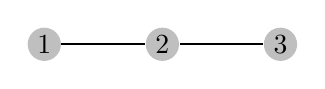
\begin{tikzpicture}[scale=1.5]
    % Draw a 7,11 network
    % First we draw the vertices
    \foreach \pos/\name in {{(1,0)/1}, {(2,0)/2}, {(3,0)/3}}
        \node[vertex] (\name) at \pos {$\name$};
    % Connect vertices with edges 
    \foreach \source/ \dest in {1/2, 2/3}
        \path[edge] (\source) -- (\dest) ;
        
\end{tikzpicture}
\end{center}

Suppose $k=n=3$. Note that after nature moves, player 2 can observe $\theta$.  We can construct an APEX equilibrium as follows.

\begin{itemize}
\item After nature moves, Rebel 2 chooses $\textbf{revolt}$ if he observes $\theta=(Rebel,Rebel,Rebel)$, and plays \textbf{revolt} in current period. Otherwise, he chooses \textbf{stay} and keeps playing \textbf{stay} afterwards. 
\item After nature moves, Rebel 1 and Rebel 3 play \textbf{stay}.
\item If Rebel 2 chooses \textbf{revolt} in the last period, then Rebel 1 (or Rebel 3) plays \textbf{revolt} in current period; if Rebel 2 chooses \textbf{stay} in the last period, then Rebel 1 (or Rebel 3) keeps playing \textbf{stay} afterwards. 
\item If a Rebel deviates from the above strategy, he will play \textbf{stay} forever; if a Rebel detects a deviation, he will also play \textbf{stay} forever.
\end{itemize}

Given the prior has full support, the above strategies constitute an equilibrium  whenever $\delta\in (\frac{1}{2},1)$. In the equilibrium path, Rebel 1 and Rebel 3 believe that $\#[Rebels](\theta)\geq 3$ with probability one if they observe that Rebel 2 has played \textbf{revolt}; believe that $\#[Rebels](\theta)< 3$ with probability one if Rebel 2 has played \textbf{stay}. Off the equilibrium path, beliefs are arbitrary.
\end{example}



In the following sections, I look for APEX equilibria for general settings.

\section{Equilibrium}
\label{sec:equilibrium}
\subsection{The case: $k=n$}

In Example ~\ref{ex_leading_ex}, the construction of an APEX equilibrium relies on some important features. First, since $k=n$, Rebel 2 will never play \textbf{revolt} if one of his neighbor is Inert. Thus, when Rebel 2 plays \textbf{revolt}, it must be the case that all Rebel 2's neighbor are Rebels.  Second, Rebel 1 or Rebel 3 can force Rebel 2 to play \textbf{revolt} to reveal the true state in the first period since only Rebel 2 knows the true state. Third, single Rebel's shifting to play \textbf{stay} forever is enough to punish a deviation. Here, the group punishment is not necessary. For instance, if a Rebel $i$ makes a detectable deviation, his neighbor can punish him by playing \textbf{stay} forever. This punishment is credible if Rebel $i$ who deviated also plays \textbf{stay} forever after he deviated. I then generalize the result for $k=n$ case after defining the \textit{path} in a network and \textit{connectedness}.

\begin{definition}
A path from $i$ to $j$, $i\neq j$ in an undirected network $G$ is a finite sequence $l_1,...,l_q$ such that $l_1=i, l_2\in \bar{G}_{l_1}, l_3\in \bar{G}_{l_2},...,l_q=j$ without repetition in $\{l_1,...,l_q\}$\footnote{See also P.39-P.40 in \citep{gross2005graph}}.  
\end{definition}

\begin{definition}
An undirected network is connected if and only if for all $i,j$, $i\neq j$ there is a path from $i$ to $j$. 
\end{definition}

\begin{theorem}
\label{prop:not_crowded}
In any FFCCU network, if the prior has full support on $\Theta$, then for $n$-person repeated $k$-Threshold game with parameter $k=n$ played in such network,  there is a $\delta^{*}$ such that a sequential APEX equilibrium exists whenever $\delta\in (\delta^{*},1)$.
\end{theorem}
\begin{proof}
The proof is constructive and is a generalization of Example ~\ref{ex_leading_ex}. The equilibrium strategy $\tau^{*}$ is as follows. After nature moves, a Rebel plays \textbf{revolt}  if there is no Inert neighbor; a Rebel plays \textbf{stay} forever if there is an Inert neighbor. After the first period, if such Rebel observed that his Rebel neighbors play \textbf{revolt} continuously in previous periods, he plays \textbf{revolt} in current period; otherwise, he plays \textbf{stay} forever. 

If a Rebel deviates, then he plays \textbf{stay} forever. If a Rebel detected a deviation, then he plays \textbf{stay} forever.

According to $\tau^{*}$, at period $s$, if a Rebel has not detected a deviation but such Rebel observed his Rebel neighbors have played \textbf{stay} once in previous periods, he forms a belief, ~$\sum_{\theta:\#[Rebels](\theta)\geq k}\beta^{\pi,\tau^*}_{G_i}(\theta|h^{s^{'}}_{G_i})=0$ for all $s^{'}\geq s$. According to this belief, playing \textbf{stay} for all $s^{'} \geq s$ is the best response. If a Rebel detects a deviation, or if he deviates to play \textbf{stay}, play \textbf{stay} is the best response since at least one of his neighbors will play \textbf{stay}. 

Since the network is FFCCU, there is a finite time $t^{s}_{\theta}$ such that all Rebels play \textbf{revolt} forever if $\#[Rebels](\theta)\geq k$; and there is a finite time $t^f_{\theta}$ such that all Rebel play \textbf{stay} forever if $\#[Rebels]< k$ in the equilibrium path. If a Rebel deviates from equilibrium path, he at most gets 0 after $\max\{t^{s}_{\theta},t^f_{\theta}\}$, while he gets $1$ after $t^{s}_{\theta}$; get $0$ after $t^f_{\theta}$. Due to the full support assumption, he will not deviate if $\sum_{\theta:\#[Rebels](\theta)\geq k}\beta^{\pi,\tau^*}_{G_i}(\theta|h^{s}_{G_i})>0$ at period $s$, otherwise he has a loss in expected continuation pay-off by $\delta^{t^s_{\theta}}\frac{\sum_{\theta:\#[Rebels](\theta)\geq k}\beta^{\pi,\tau^*}_{G_i}(\theta|h^{s}_{G_i})}{1-\delta}$ after $t^s_{\theta}$. There is a $0<\delta^{*}<1$ such that he will not deviate whenever $\delta\in (\delta^{*},1)$.

To check if $\tau^{*}$ and $\{\beta^{\pi,\tau^*}_{G_i}(\theta|h^{s}_{G_i})\}_{i\in N, h^{s}_{G_i}\in H^{s}_{G_i},s\geq 1}$ satisfy full consistency\footnote{Krep and Wilson (1982)}, take any $\eta\in (0,1)$ such that Rebels play $\tau^{*}$ with probability $1-\eta$, and play any other strategy with probability $\eta$. Clearly, when $\eta \rightarrow 0$, the beliefs converges to $\{\beta^{\pi,\tau^*}_{G_i}(\theta|h^{s}_{G_i})\}_{i\in N, h^{s}_{G_i}\in H^{s}_{G_i},s\geq 1}$ for all $i\in N, h^{s}_{G_i}\in H^{s}_{G_i},s\geq 1$.
\end{proof}



\subsection{The cases : $1<k<n$}

The above equilibrium construction in the proof of Theorem ~\ref{prop:not_crowded} may not constitute an equilibrium for $k<n$ cases. First, a Rebel still has incentive to play \textbf{revolt} even if there is an Inert neighbor. Second, an Inert never transmit additional information about relevant information since they have only one action. We then require more assumptions on the priors to get an APEX equilibrium. Example ~\ref{ex_strong_connectedness} shows that, without additional assumptions, the game might be reduced to an incomplete information game without communication, and thus an APEX equilibrium does not exist.

\begin{example}\label{ex_strong_connectedness}
Let $k=2$ and let the network be the following. Assume $\theta=(Rebel_1,Inert_2,Rebel_3)$.

\begin{center}
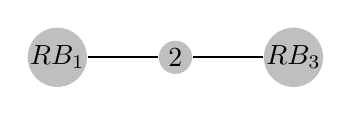
\begin{tikzpicture}[scale=1.5]
    % Draw a 7,11 network
    % First we draw the vertices
    \foreach \pos/\name in {{(1,0)/RB_1}, {(2,0)/2}, {(3,0)/RB_3}}
        \node[vertex] (\name) at \pos {$\name$};
    % Connect vertices with edges 
    \foreach \source/ \dest in {RB_1/2, 2/RB_3}
        \path[edge] (\source) -- (\dest) ;
        
\end{tikzpicture}
\end{center}

First, since $k=2$, Rebel 1 has incentive to play \textbf{revolt} when $\pi(\{\theta:\theta_3=Rebel\})$ is high enough given that Rebel 3 will play revolt. Second, Rebel 1 never learn $\theta_3$ since Inert 2 can not reveal information about $\theta_3$. We are now in an incomplete information game without communication. Clearly, an equilibrium which is APEX did not exist in this case.

\end{example}

I narrow down the priors to exclude cases similar  to Example ~\ref{ex_strong_connectedness}. I will define \textit{Strong connectedness} and \textit{Full support on strong connectedness} as follows.

\begin{definition}
\textbf{Strong connectedness}: Given $G$, a state $\theta$ has strong connectedness if and only if for every pair of Rebels, there is a path consisting of Rebels to connect them.
\end{definition}  

\begin{definition}
\textbf{Full support on strong connectedness}: Given $G$, $\pi$ has full support on strong connectedness if and only if 
\[\pi(\theta)>0\Leftrightarrow \text{ $\theta$ has strong connectedness }\] 
\end{definition}  


The goal of this paper is to show that a weak sequential APEX equilibrium always exists in acyclic FFCCU networks whenever $\delta$ is sufficiently high. I define \textit{acyclic} in the following definition and state my main theorem in Theorem ~\ref{thm_main_result}. 
\begin{definition}
A FFCCU network is acyclic $\Leftrightarrow$ the path from $i$ to $j$ is unique for all $i\neq j$, . 
\end{definition}

\begin{theorem}
\label{thm_main_result}
In any acyclic FFCCU network, if $\pi$ has full support on strong connectedness, then for $n$-person repeated $k$-Threshold game with parameter $1\leq k < n$ played in networks, there is a $\delta^{*}$ such that a weak sequential APEX equilibrium exists whenever $\delta\in(\delta^{*},1)$.
\end{theorem}

The equilibrium in Theorem ~\ref{thm_main_result} is constructive. According to definition ~\ref{Def_expost_efficient}, I will construct the equilibrium path first, then construct the in-path and off-path beliefs, and then check if the strategies and belief system indeed constitute an equilibrium. I begin with an overview of the main ideas, and then illustrate how such construction works. The whole equilibrium strategies and all the omitted proofs are in the Appendix.  

\subsubsection{Overview}

Given that the state has strong connectedness, Rebels have to find a way to communicate with each other. The construction of APEX is not trivial because the ``dimension'' of information is generally higher than the cardinality of their own action space. Rebels then use several sequences of actions to transmit information, and thus we have to track the belief updating in the horizontal time line and to check if such sequences constitute equilibrium strategies. To see that a Rebel needs to communicate about higher-dimension information, let's compare Example ~\ref{ex_cycle_number_5} and Example ~\ref{ex_cycle_number_6}.


\begin{example}\label{ex_cycle_number_5}
Let $k=5$. Let the network and the state $\theta$ be the following.

\begin{center} 
  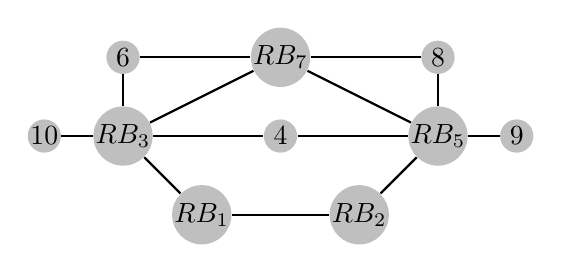
\begin{tikzpicture}[scale=1]
    % First we draw the vertices
    \foreach \pos/\name in {{(2,1)/RB_1}, {(4,1)/RB_2}, {(1,2)/RB_3}, {(5,2)/RB_5}, {(3,3)/RB_7}, {(3,2)/4}, {(1,3)/6}, {(5,3)/8}, {(6,2)/9}, {(0,2)/10}}
        \node[vertex] (\name) at \pos {$\name$};
        
%        \foreach \pos/\name in {{(3,2)/4_L}, {(1,3)/6_L}, {(5,3)/8_L}, {(6,2)/9_L}, {(0,2)/10_L}}
%   \node[selected vertex] (\name) at \pos {$\name$};
    
    % Connect vertices with edges 
    \foreach \source/ \dest in {RB_1/RB_2, RB_1/RB_3, RB_2/RB_5, RB_3/4, RB_3/6, RB_3/RB_7, 4/RB_5, RB_5/RB_7, RB_5/8, RB_5/9,6/RB_7, RB_7/8, RB_3/10}
        \path[edge] (\source) -- (\dest) ;
\end{tikzpicture}
\end{center} 

\end{example}


\begin{example}\label{ex_cycle_number_6}
Let $k=6$. Let the network and the state $\theta$ be the following.
\begin{center} 
  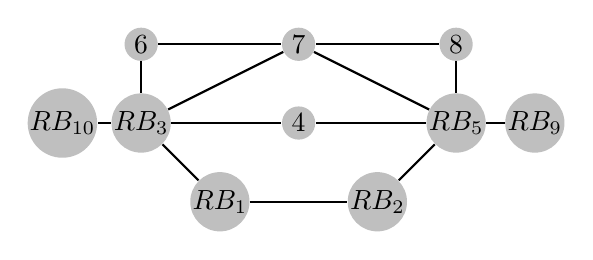
\begin{tikzpicture}[scale=1]
    % First we draw the vertices
    \foreach \pos/\name in {{(2,1)/RB_1}, {(4,1)/RB_2}, {(1,2)/RB_3}, {(5,2)/RB_5}, {(3,3)/7}, {(3,2)/4}, {(1,3)/6}, {(5,3)/8}, {(6,2)/RB_9}, {(0,2)/RB_{10}}}
        \node[vertex] (\name) at \pos {$\name$};
        
%        \foreach \pos/\name in {{(3,2)/4_L}, {(1,3)/6_L}, {(5,3)/8_L}, {(6,2)/9_L}, {(0,2)/10_L}}
%   \node[selected vertex] (\name) at \pos {$\name$};
    
    % Connect vertices with edges 
    \foreach \source/ \dest in {RB_1/RB_2, RB_1/RB_3, RB_2/RB_5, RB_3/4, RB_3/6, RB_3/7, 4/RB_5, RB_5/7, RB_5/8, RB_5/RB_9,6/7, 7/8, RB_3/RB_{10}}
        \path[edge] (\source) -- (\dest) ;
\end{tikzpicture}
\end{center} 


\end{example}

There are 6 Rebels in Example ~\ref{ex_cycle_number_6}, while there are 5 Rebels in Example ~\ref{ex_cycle_number_5}. Let's suppose we have a ``talking strategy'' as follows. Rebel 3 and Rebel 5 can talk about ``how many Rebels in their neighborhood'' to Rebel 1 and Rebel 2. Rebel 1 and Rebel 2 then talk with each other about ``how many Rebels they have known'' conditional on Rebel 3 and Rebel 5's talking. In this scenario, Rebel 1 and Rebel 2 cannot know how many Rebels are present since Rebel 3 and Rebel 5 will reveal the same number of Rebels in both examples. Thus, ``talking about how man nearby Rebels'' is not enough to reveal the information, Rebels have to talk about other Rebels' identities. 

Another difficulty is that higher-order beliefs are hard to be tracked.  Although Lemma ~\ref{lemma_learn} shows that there is a timing such that each Rebel can learn the relevant information, but Lemma ~\ref{lemma_learn}  did not characterize how Rebels commonly learn when is that timing. This higher-order information about ``Have some Rebels learned the relevant information?'' is an apparently giant object in the private monitoring repeated game. Here, Rebels use several sequences to communicate about this information and coordinate their continuation actions if they can commonly know the relevant information.

I construct an APEX equilibrium with a weaker sequential consistency by using an off-path belief. This off-path belief serves as  a grim-trigger. More specifically, if a Rebel detects a deviation, he forms the belief of $\sum_{\theta \in \{\theta:\theta_j=Inert,j\notin G_i\}}\beta^{\pi,\tau}_{G_i}({\theta}|h^{s^{'}}_{G_i})=1$ for all $s^{'}\geq s$. I.e., he will believe that all players outside his neighborhood are Inerts. Thus, if he has less than $k$ Rebel neighbors, he will play \textbf{stay} afterwards. 

The equilibrium is constructed through several steps. I organized those steps by following three subsections. In the first subsection, I define \textit{information hierarchy in $G$} that determines which Rebels should transmit their private information in equilibrium. In the second subsection, I display Rebels' strategies in the equilibrium path and show the belief updating in the path. Finally, I discuss off-path belief in subsection three and give a sketch of the proof for Theorem ~\ref{thm_main_result}. 

\subsubsection{Step 1. Information hierarchy in $G$}

The information hierarchy is defined on a network $G$ after nature chooses a state but before the game is played. I will use the term ``node $i$'' instead of ``player $i$'' in this step. 

I define information hierarchy by defining $\{N^{-1}_i,N^{0}_i, N^{1}_i...\}$ and $\{I^{-1}_i,I^{0}_i, I^{1}_i...\}$ for each $i\in N$, and then define $\{\leq^0, \leq^1, \leq^2\}$ and $\{R^0,R^{1}, R^{2}...\}$ for each iteration in $(0,1,2,...)$. I use the term ``blocks'' to represent the ``iterations'', since the term, \textit{block}, will be used as a terminology when I display in-the-path equilibrium strategies later. 

Given $\theta$, I define information hierarchy as follows.
\begin{itemize}

\item \textbf{0-block}
Let
\begin{eqnarray*}
N^{-1}_i &\equiv &  i \\
I^{-1}_i & \equiv & i
\end{eqnarray*}

Then define $R^0$ as 
\begin{equation}
R^0\equiv\{i:\theta_i\in[Rebels](\theta)\}
\end{equation}

\item \textbf{1-block}
Let
\begin{eqnarray*}
N^0_i &\equiv &  G_i \\
I^0_i & \equiv & G_i\cap R^0
\end{eqnarray*}

Define the set $\leq^0$ by defining
\begin{equation}i\in \leq^0 \Leftrightarrow \exists  j\in \bar{G}_i [I^0_i\subseteq N^0_j\cap R^0]\end{equation}  

Then define $R^1$ as 
\begin{equation}
R^{1} \equiv \{i\in R^0|i\notin \leq^0\}
\end{equation}

\item \textbf{$t+1$-block, $t\geq 1$}
Let
\begin{eqnarray*}
N^t_i & \equiv & \bigcup_{k\in I^{t-1}_i}G_k \\
I^t_i & \equiv & \bigcup_{k\in G_i\cap R^t}I^{t-1}_k
\end{eqnarray*}


Define the set $\leq^t$ by defining
\begin{equation}i\in \leq^t \Leftrightarrow \exists j\in \bar{G}_i[I^t_i\subseteq N^t_j\cap R^0]\end{equation}

Then define $R^{t+1}$ as 
\begin{equation}
R^{t+1} \equiv  \{i\in R^t|i\notin \leq^t\}
\end{equation}


\end{itemize}

Thus, by examining the definition of $\leq^t$, $R^t$ nodes are those nodes who have information about some other Rebels' existence while none of their neighbors have such information. At $t$-block, $R^t$ nodes have the information, $I^{t-1}$, which contains the updated information as the union of his $R^{t-1}$ neighbors' information, $I^{t-2}$. 

Since communication may incur expected costs, if a Rebel's private information can be fully reported by his neighbors while there is no punishment schema, then he has no incentives to report it. In each $t\geq 1$-block, non-$R^t$ nodes are those node whose information can be fully reported by some of his Rebel neighbors. By defining information hierarchy, I implicitly characterize Rebels' incentives in reporting information. If the networks are acyclic, Theorem ~\ref{lemma_empty} shows that it is sufficient to let only $R^t$ nodes report information while non-$R^t$ are not needed. 
\begin{theorem}
\label{lemma_empty}
If the network is FFCCU without cycle and if the state has strong connectedness, then 
\[R^0\neq \emptyset \Rightarrow \exists t\geq 0[\exists i\in R^t[I^t_i=R^0]]\]
\end{theorem}



\subsubsection{Step 2: Equilibrium strategies in the path}


First, I assigned each player a distinguished prime number. Such indexation is starting from $3$. I index players $(1,2,...,n)$ as $(3,5,...,x_n)$ where $x_n$ is a prime number and the prime number assigned to $i$ will be $x_i$. Since the multiplication prime numbers can be uniquely de-factorized, I use this property to let Rebels report the information about other Rebels' existence by reporting the multiplication of those Rebels' prime numbers.

I let $\langle\rangle$ denote a sequence and let $\bar{N}\subset N$ denote an non-empty subset of $N$. Table ~\ref{Table_msg_form} shows my notations in indicating some forms of sequences. 

\begin{table}[t]
\caption{Notations}
\label{Table_msg_form}
\begin{center}
\begin{tabular}{l c c}
$\bar{N}$ 										& $\equiv$ 			& a non-empty subset of $N$  \\
$x_i$ 											& $\equiv$ 			& node $i$'s prime-number index  \\
$X_{\bar{N}}$ 								& $\equiv$ 			& $\prod_{j\in \bar{N}}x_j$  \\
\textbf{s}										& $\equiv$ 			& \textbf{stay}  \\
\textbf{r}										& $\equiv$ 			& \textbf{revolt}  \\
$\langle \textbf{stay} \rangle$ 		& $\equiv$ 			& $\langle \textbf{s},...,\textbf{s}\rangle$  \\
$\langle \textbf{revolt} \rangle$ 	& $\equiv$ 			& $\langle \textbf{r},...,\textbf{r}\rangle$  \\
$\langle  \bar{N} \rangle$ 				& $\equiv$ 			& $\langle \textbf{s},...,\textbf{s},\underbrace{\textbf{r},\textbf{s},...,\textbf{s}}_{X_{ \bar{N}}}\rangle$  \\

$\langle 1 \rangle$	 					& $\equiv$ 			& $\langle \textbf{s},...,\textbf{s},\underbrace{\textbf{r}}_{1}\rangle$  \\
$\langle x_i \rangle$	 	& $\equiv$ 			& $\langle \textbf{s},...,\textbf{s},\underbrace{\textbf{r},\textbf{s},...,\textbf{s}}_{x_i}\rangle$  \\
\end{tabular}
\end{center}
\end{table}

I let $|\langle\rangle|$ denote the length of a sequence. The form and the length of a sequence determine a sequence. For instance, if a sequence takes the form $\langle 1 \rangle$ and if its length is three (i.e., $|\langle 1 \rangle|=3$), then this sequence is $\langle \textbf{s},\textbf{s},\textbf{r}\rangle$. Note that the length of a form is calculate from the end of such sequence.

In the equilibrium path, two phases, {reporting period} and {coordination period}, alternate as follows.
\[\underbrace{<\text{coordination period}>}_{0-block}\underbrace{<\text{reporting period}><\text{coordination period}>}_{1-block}...\]
I.e., after nature chooses a state, all the Rebels start with $0$-block, then enter to $1$-block,...,and so on. $0$-block has only one period, coordination period. The $t$-blocks, $t\geq 1$ has two periods, reporting period and coordination period. The length of a phase is finite.

I call a sequence a {reporting messages} ({resp.} {coordination messages}) if such sequence is played in reporting period ({resp.} coordination period). In reporting period in each $t\geq 1$-block, Rebels use the sequences listed in Table ~\ref{Table_msg_reporting} to report their current information about $\theta$. In coordination period in each $t\geq 0$-block , Rebels use the sequences listed in Table ~\ref{Table_msg_coordination} to check if there are some Rebels have known the relevant information. After the coordination period, they either start to coordinate or enter at the next reporting period. 

I begin to illustrate these messages as follows.



\subsubsection*{Reporting messages in reporting period}

Let $|\langle RP^t \rangle|$ be the length of reporting period in $t$-block.  In the equilibrium path, I construct those strategies that can induce some special sequences with length $|\langle RP^t \rangle|$. Table ~\ref{Table_msg_reporting} lists those special sequences. Any other sequence will be considered as a deviation. 

\begin{table}[ht]
\caption{Reporting messages}
\label{Table_msg_reporting}
\begin{center}
\begin{tabular}{c c }
Reporting Messages 		&   \\
\hline
$\langle  \textbf{stay} \rangle$ 	& 	 \\
$\langle  {I^{t-1}_i} \rangle$ 		&   \\
$\langle 1 \rangle$ 		             &    
\end{tabular}
\end{center}
\end{table}

Table ~\ref{Table_blf_up_reporting} shows Rebel $j$'s in-the-path belief updating given his neighbor $i$'s reporting messages.


\begin{table}[ht]
\caption{Belief updating after reporting period}
\label{Table_blf_up_reporting}
\begin{center}
\begin{tabular}{l c l}
$i$ plays 		&  			& The events $j\in \bar{G}_i$ believe with probability one  \\
\hline
$\langle  \textbf{stay} \rangle$ 	& 			    & $i\notin R^t$  \\
$\langle  {I^{t-1}_i} \rangle$ 		&  			& $i\in R^t$ and $\theta_l=Rebel$ if $l\in I^{t-1}_i$      \\
$\langle 1 \rangle$ 		             &  			& $i\in R^t$ and $i$ has known $\#[Rebels](\theta)\geq k-1$ \\
\end{tabular}
\end{center}
\end{table}

Table ~\ref{Table_blf_up_reporting} shows that a Rebel can tell whether or not his neighbor is a $R^t$ after the reporting period. Recall that $R^t$ Rebels have the information about other Rebel's existence, which any of their neighbor does not have. If Rebel $j$ has observed that all of his neighbors are not $R^t$, then he is sure that $\#[Rebels](\theta)< k$ if $\#I^{t-1}_j<k$. 

The important feature here is that $\langle 1 \rangle$ is introduced. $\langle 1 \rangle$ serves as a signal to indicate a ``pivotal player'' and to solve potential free rider problems. I elaborate this feature by providing some examples. First, free rider problems may occur if $\langle 1 \rangle$ is not introduced. Let's consider the following Example ~\ref{ex_free_rider_tree}.

\begin{example} \label{ex_free_rider_tree}\textbf{Free Rider Problem}

Let $k=5$ and assume that there are messages, $\langle M_4 \rangle$ and $\langle M_5 \rangle$, for Rebel 4, 5. To simply the analysis, let players play the game starting from a reporting period. Further, suppose that Rebels will play \textbf{revolt} forever after observing $\langle M_4 \rangle$ or $\langle M_5 \rangle$ \footnote{played by Rebel 4 or 5 immediately after such reporting period}; otherwise they will play \textbf{stay} forever. Let $G$ be the following.

\begin{center}
\begin{tikzpicture}[scale=1]
    % Draw a 7,11 network
    % First we draw the vertices
    \foreach \pos/\name in {{(1,2)/RB_1}, {(2,1)/RB_2}, {(2,3)/3}, {(3,2)/RB_4}, {(4,2)/RB_5}, {(5,1)/6}, {(5,3)/7}, {(6,2)/RB_8}}
        \node[vertex] (\name) at \pos {$\name$};
    
    
    % Connect vertices with edges 
    \foreach \source/ \dest in {RB_1/4, RB_2/RB_4,3/RB_4,RB_4/RB_5, RB_5/6, RB_5/7, RB_5/RB_8}
        \path[edge] (\source) -- (\dest) ;
        
\end{tikzpicture}
\end{center}

Note that Rebel 4 and Rebel 5 are $R^1$ members. Let $\langle \rangle_4$ and $\langle \rangle_5$ are the sequences of actions they may use to report their Rebel neighbors' positions. If Rebel 5 report truthfully, since Rebel 4 can use $\langle M_4 \rangle$ to initialize the coordination, Rebel 4 will not report truthfully by arranging the occurrence of \textbf{revolt}s. The same argument can be applied to Rebel 5. Therefore, both of Rebel 4 and Rebel 5 will not report truthfully.

\end{example}

Two sources constitute the free rider problem in the above example. The first is that messages, $\langle M_4 \rangle$ and $\langle M_5 \rangle$, can coordinate Rebels' future actions regardless what reporting messages used. The second is that Rebel 4 and Rebel 5 are sure that they will learn the state given others' truthful reporting. In other words, Rebel 4 and Rebel 5 are ``pivotal''. To see the latter source more clearly, let's consider the following Example ~\ref{ex_pivotal_1}.



\begin{example} \label{ex_pivotal_1}\textbf{Pivotal player: Case 1}
Let $k=6$ and suppose that there are message, $\langle M_3 \rangle,\langle M_5 \rangle$, and $ \langle M_7 \rangle$, for Rebel 3,5,7 to initiate a coordination. Let players play the game starting from a reporting period. Further, suppose Rebel will play \textbf{revolt} forever after observing $\langle M_3 \rangle$, $\langle M_5 \rangle$, or $\langle M_7 \rangle$ \footnote{immediately after this reporting period}; otherwise they will play \textbf{stay} forever. Let $G$ be the following.
\begin{center}
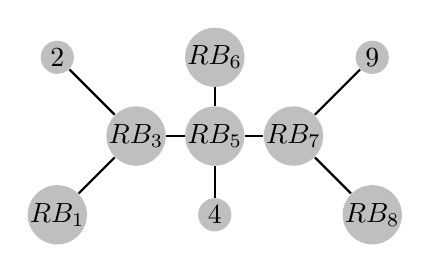
\begin{tikzpicture}[scale=1]
    % Draw a 7,11 network
    % First we draw the vertices
    \foreach \pos/\name in {{(1,1)/RB_1}, {(1,3)/2}, {(2,2)/RB_3}, {(3,1)/4}, {(3,2)/RB_5}, {(3,3)/RB_6}, {(4,2)/RB_7}, {(5,1)/RB_8}, {(5,3)/9}}
        \node[vertex] (\name) at \pos {$\name$};
    
    
    % Connect vertices with edges 
    \foreach \source/ \dest in {RB_1/RB_3, 2/RB_3,RB_3/RB_5,4/RB_5, RB_6/RB_5, RB_5/RB_7, RB_7/RB_8, RB_7/9}
        \path[edge] (\source) -- (\dest) ;
        
\end{tikzpicture}
\end{center}

Note that Rebel 3, 5, 7 are $R^1$ members. In contrast to Example ~\ref{ex_free_rider_tree}, Rebel 3 and Rebel 7 still have incentive to report truthfully. Suppose they did not report truthfully, there is a possibility such that Rebel 5 will misunderstand the state. Since they are not sure if they can learn the state after the reporting period, and since the coordination to \textbf{revolt} has to be initiated after this reporting period, they have incentive to report truthfully.

Rebel 5, however, has no incentive to report truthfully given others' truthful reporting since Rebel 5 is sure that he will know the true state immediately after reporting period.
\end{example}
   
Combine the discussions in Example ~\ref{ex_free_rider_tree} and Example ~\ref{ex_pivotal_1} , a way to deal with the free rider problem is to let one of Rebels involved in this problem be a free rider while letting the others report truthfully. If the networks are FFCCU without cycles, Lemma ~\ref{lemma_at_most_two_nodes} shows that the free rider problem can be identified before the game enter to $t$-block. More precisely, first define $Tr_{ij}$ as a tree rooted in $i$ with leaves spanning from $j\in \bar{G}_i$.

\begin{definition}
$Tr_{ij}\equiv \{l\in N:\text{there is a unique path $\{l,...,j,i\}$ from $l$ to $i$ through $j$}\}$
\end{definition}

Let $C^t$ be those $R^t$ nodes such that there are no possible Rebels connecting with them by a path consisting of more than three Rebels. I.e., 
\[C^t=\{i\in R^t:\nexists j\in R^{t-1}\cap \bar{G}_i[\exists l,l^{'}\in Tr_{ij}[l\in N^{t-1}_j\backslash I^{t-1}_i \text{ and } l^{'}\in \bar{G}_l]]\}\]
.  For instance, Rebel 4 and Rebel 5 in Example ~\ref{ex_free_rider_tree} are $C^1$ nodes, and Rebel 5 in Example ~\ref{ex_pivotal_1} is also a $C^1$ node. Then we can show the following lemmas. 

\begin{lemma}
\label{lemma_at_most_two_nodes}
If the network is FFCCU without cycle, and  if the state has strong connectedness, then for each $t$-block
\begin{enumerate}
\item $0\leq |C^t| \leq 2$.
\item Moreover, suppose there are two nodes in $C^t$, then they are each other's neighbor.
\end{enumerate}
\end{lemma}


\begin{lemma}
\label{lemma_no_node_outside}
If the network is FFCCU without cycle, and if the state has strong connectedness, then 
\[i\in C^t \Rightarrow \text{there is no possible Rebel node outside of }\bigcup_{k\in N^{t-1}_i}G_k\]
for each $t$-block.
\end{lemma}

According to Lemma ~\ref{lemma_at_most_two_nodes}, $C^t$-nodes can identify each other by the following procedures: First, a $C^t$-node ,$j$, assumes that one of his $R^{t-1}$ neighbor, $i$, is a $R^t$-node. Second, he checks if $i$ is in $C^t$ by the definition of $C^t$. Third, if $i$ is identified as a $C^t$ node, $i,j$ are the only $C^t$ nodes. Finally, he assumes that $i$ will do the same procedure to identify him. Since $j$ is a $C^t$-node, $i$ must be able to identify him if $i$ is a $C^t$-node, and thus both $C^t$-nodes can identify each other.

If there is more than one $C^t$ node, I let the smaller prime-indexed node be a free rider while letting the other one report truthfully.

However, Lemma ~\ref{lemma_no_node_outside} does not show that $C^t$-nodes are the only pivotal Rebels. Some pivotal Rebels cannot be identified before the game enters at $t$-block. We have to identify them during reporting period, and therefore we have to track their information updating sequentially. These other pivotal Rebels are those Rebel who are sure that they will learn the relevant information, \textit{$\#[Rebels](\theta)\geq k$ or $\#[Rebels](\theta)< k$}, after reporting period. Example ~\ref{ex_pivotal_2} is a concrete example.

\begin{example} \label{ex_pivotal_2}\textbf{Pivotal player: Case 2}
Let $k=6$. Again, assume that there are coordination messages $\langle M\rangle$s for Rebels. Let players play the game starting from a reporting period. Again, let's suppose Rebel will play \textbf{revolt} forever after observing $\langle M \rangle$ played \footnote{It requires four periods to let the coordination message transmit.} after that reporting period; otherwise they will play \textbf{stay} forever. Let $G$ be the following.

\begin{center}
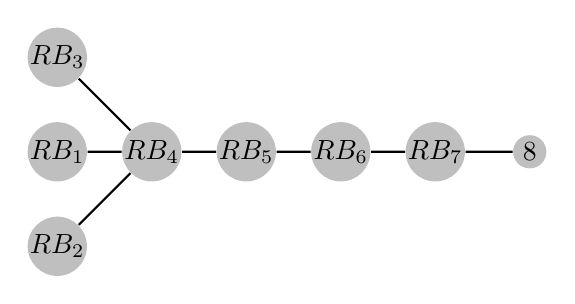
\begin{tikzpicture}[scale=1.2]
    % Draw a 7,11 network
    % First we draw the vertices
    \foreach \pos/\name in {{(2,2)/RB_1}, {(2,1)/RB_2}, {(2,3)/RB_3}, {(3,2)/RB_4}, {(4,2)/RB_5}, {(5,2)/RB_6}, {(6,2)/RB_7}, {(7,2)/8}}
        \node[vertex] (\name) at \pos {$\name$};
    
    
    % Connect vertices with edges 
    \foreach \source/ \dest in {RB_1/RB_4, RB_2/RB_4,RB_3/RB_4,RB_4/RB_5, RB_5/RB_6, RB_6/RB_7, RB_7/8}
        \path[edge] (\source) -- (\dest) ;
        
\end{tikzpicture}
\end{center}

In this case, no Rebels are in $C^1$, but Rebel 4 will deviate from reporting $\langle I^0_4 \rangle$. Note that Rebel 4 has already known there are 5 Rebels. If node 6 is a Rebel, Rebel 5 will report that, and therefore he will know $\#[Rebels](\theta)\geq 6$; Otherwise, due to the state has strong connectedness, Rebel 5 will report nothing, and then he will know $\#[Rebels](\theta)< 6$. Since he can use the message $\langle M \rangle$ to initiate the coordination, his deviation is profitable for him.
\end{example}

After discussing above examples, the message $\langle 1 \rangle$ is introduced. In the equilibrium path (shown in the Appendix), there are two kinds of pivotal Rebels. One kind are those Rebels who have already learned that $k-1$ are present before they report their information. The other kinds are those Rebels in $C^t$. The pivotal Rebels will play $\langle 1 \rangle$ in the equilibrium path. The in-the-path beliefs after observing $\langle 1 \rangle$ are then to believe that \textit{some Rebels has known $\#[Rebels](\theta)\geq k-1$}, as Table ~\ref{Table_blf_up_reporting} shows.




\subsubsection*{Coordination messages in coordination period}

As previous examples show, the ignorance of reporting messages after observing a coordination message, says $\langle M \rangle$, may incur untruthfully reporting. I introduce $\langle 1 \rangle$ to tackle this issue. However, the combination of these two messages, $\langle 1 \rangle\langle M \rangle$, is another ``coordination message''. I.e., $\langle\langle \textbf{s}, \textbf{r} \rangle\langle M \rangle\rangle$ is another coordination message by truncating previous actions in $\langle 1 \rangle$ and concatenating the remaining sequence to $\langle M \rangle$. If continuation actions after observing $\langle\langle \textbf{s}, \textbf{r} \rangle\langle M \rangle\rangle$ are regardless of what previous actions in reporting period, the issue of untruthfully reporting still exists. In this section, I deal with this issue by letting continuation actions be contingent on not only coordination messages but also  reporting messages.


There are three divisions in coordination period and there are several sub-blocks in each division. In $t=0$ block, the structure is
\[\overbrace{\langle\underbrace{\langle \cdot \rangle }_{\text{$1$ sub-block}}\rangle}^{\text{1st division}} \overbrace{\langle\underbrace{\langle \cdot \rangle }_{\text{$1$ sub-blocks}} \rangle}^{\text{2nd division}} \overbrace{\langle\underbrace{\langle \cdot \rangle \cdot \cdot \cdot \langle \cdot \rangle}_{\text{$n$ sub-blocks}}\rangle}^{\text{3rd division}}\] 
; in $t>0$ blocks, the structure is
\[\overbrace{\langle\underbrace{\langle \cdot \rangle \cdot \cdot \cdot \langle \cdot \rangle}_{\text{$n$ sub-blocks}}\rangle}^{\text{1st division}} \overbrace{\langle\underbrace{\langle \cdot \rangle \cdot \cdot \cdot \langle \cdot \rangle}_{\text{$t+1$ sub-blocks}} \rangle}^{\text{2nd division}} \overbrace{\langle\underbrace{\langle \cdot \rangle \cdot \cdot \cdot \langle \cdot \rangle}_{\text{$n$ sub-blocks}}\rangle}^{\text{3rd division}}\] 
.


Let $CD^t_{m,q}$ be the $m$ sub-block in $q$ division, and let $|\langle CD^t_{m,q} \rangle|$ be the length of $CD^t_{m,q}$.  In the equilibrium path, outcomes of strategies take the following forms of sequences with length $|\langle CD^t_{m,q} \rangle|$. Table ~\ref{Table_msg_coordination} shows those forms.
\begin{table}[ht]
\caption{Coordination messages}
\label{Table_msg_coordination}
\begin{center}

\begin{tabular}{cc }
Coordination messages		&   \\
\hline
$\langle x_i \rangle$ 	& 	 \\
$\langle \textbf{stay} \rangle$	&   \\
\textbf{r}									& 	\\
\textbf{s}									& 	\\
\end{tabular}
\end{center}
\end{table}

In my construction, all the Rebels will play \textbf{revolt} after $0$-block if there is a Rebel who has $k$ or more Rebels neighbors. In this subsection, I will focus on displaying the behaviors in $t>0$ block since $0$-block has a simpler structure,. The whole equilibrium path is shown in the Appendix.

After $CD^t_{1,1}$, the belief formed by Rebel $j$ after observing neighbor $i$'s behavior in equilibrium path is shown in Table ~\ref{Table_blf_up_cdt11}. Table ~\ref{Table_blf_up_cdt11} shows that Rebel $j$ can tell the information of the event, $\{\theta:\#[Rebels](\theta)< k\}$. Clearly, $j$ will play \textbf{stay} forever if he believes that this event happens with probability one.

In the first division, Rebels play $\langle x_i \rangle$ unless they observe $\langle \textbf{stay} \rangle$ as Table ~\ref{Table_stg_cdt21} and Table ~\ref{Table_stg_cdtm1} shows. After $CD^t_{n,1}$, the information about $\#[Rebels](\theta)< k$ will be transmitted across Rebels. 
\begin{table}[ht]
\caption{Belief updating after $CD^t_{1,1}$, $t>0$}
\label{Table_blf_up_cdt11}
\begin{center}
\begin{tabular}{c c c}
In $RP^t$ 	&  	In $CD^t_{1,1}$		&  \\
\hline
\hline
$i$ plays 		&  	$i$ plays		& The events $j\in \bar{G}_i$ believes with probability one  \\
\hline
$\langle  \textbf{stay} \rangle$ 	& 	$\langle x_i \rangle$	    & $i\notin R^t$ \\
$\langle  {I^{t-1}_i} \rangle$ 		&  $\langle \textbf{stay} \rangle$		& $\#[Rebels](\theta)< k$     \\
$\langle  {I^{t-1}_i} \rangle$ 		&  $\langle x_i \rangle$		& $i\in R^t$     \\
$\langle 1 \rangle$ 		             &  $\langle \textbf{stay} \rangle$		& $\#[Rebels](\theta)< k$  \\
$\langle 1 \rangle$ 		             &  $\langle x_i \rangle$		&  $\#[Rebels](\theta)\geq k$ 
\end{tabular}
\end{center}
\end{table}



\begin{table}[ht]
\caption{In-path strategies in $RP^t$, $CD^t_{1,1}$, and $CD^t_{2,1}$, $t>0$}
\label{Table_stg_cdt21}
\begin{center}
\begin{tabular}{c c c}
In $RP^t$ 	 	&  	In $CD^t_{1,1}$		&  In $CD^t_{2,1}$	\\
\hline
\hline
$i$ plays 		  							&  	$i$ plays									& $j\in \bar{G}_{i}$ plays  \\
\hline
$\langle  \textbf{stay} \rangle$ 	& 	$\langle x_i \rangle$	    & $\langle x_i \rangle$ \\
$\langle  {I^{t-1}_i} \rangle$ 		&  $\langle \textbf{stay} \rangle$		& $\langle \textbf{stay} \rangle$     \\
$\langle  {I^{t-1}_i} \rangle$ 		&  $\langle x_i \rangle$		& $\langle x_i \rangle$     \\
$\langle 1 \rangle$ 		             &  $\langle \textbf{stay} \rangle$		& $\langle \textbf{stay} \rangle$  \\
$\langle 1 \rangle$ 		             &  $\langle x_i \rangle$		&  $\langle x_i \rangle$  
\end{tabular}
\end{center}
\end{table}

\begin{table}[ht]
\caption{In-path strategies after $CD^t_{m,1}$, where $m\geq 2$, $t>0$}
\label{Table_stg_cdtm1}
\begin{center}
\begin{tabular}{c c c}
In $CD^t_{m,1}$, $m\geq 2$ 	 	&  	In $CD^t_{m+1,1}$,$m\geq 2$		& 	\\
\hline
\hline
$i$ plays 		  							&  $j\in \bar{G}_{i}$ plays  								& \\
\hline
$\langle x_i \rangle$ 	& 	$\langle x_i \rangle$	    &  \\
$\langle \textbf{stay} \rangle$		&  $\langle \textbf{stay} \rangle$	&  \\

\end{tabular}
\end{center}
\end{table}



In $CD^t_{1,2}$, Rebels check if the coordination to \textbf{revolt} can be initiated. Table ~\ref{Table_blf_up_cdt12} shows that $\langle \textbf{stay} \rangle$ is the coordination message to initiate the coordination to \textbf{revolt}. The important feature in Table ~\ref{Table_blf_up_cdt12} is that $\langle \textbf{stay} \rangle$ is a coordination message to \textbf{revolt} \textit{only if} $\langle  {I^{t-1}_i} \rangle$ or $\langle 1 \rangle$ has been played in reporting period.  Since this coordination message is contingent on reporting messages, initiating the coordination to \textbf{revolt} requires Rebels to report something---play \textbf{revolt} somewhere. This trade-off between ``reporting something and then coordinating to \textbf{revolt}'' and ``reporting nothing and then failing to coordinate'' enforces Rebels to report something, otherwise they have no chances to coordinate to \textbf{revolt}. Note that a Rebel is willing to initiate the coordination since $\langle \textbf{stay} \rangle$ incurs no expected cost. 

After $CD^t_{1,2}$, Rebels start to transmit the information about $\#[Rebels](\theta)\geq k$ in $CD^t_{m,2}$ $m\geq 2$ as Table ~\ref{Table_stg_cdt12} and Table ~\ref{Table_stg_cdtm2} shows. In the equilibrium path, they play $\langle \textbf{stay} \rangle$ unless they observe $\langle x_i \rangle$. After $CD^t_{{t+1},1}$, the information about $\#[Rebels](\theta)\geq k$ will be transmitted among $k$ or more Rebels. 

\begin{table}[ht]
\caption{Belief updating after $CD^t_{1,2}$, $t>0$}
\label{Table_blf_up_cdt12}
\begin{center}
\begin{tabular}{l c c c}
In $RP^t$ 	 	&  	In $CD^t_{1,1}$		&  In $CD^t_{1,2}$	  &\\
\hline
\hline
$i$ plays 		                             &  	$i$ plays		&				$i$ plays			& The events $j$ believes with probability one  \\
\hline
$\langle  \textbf{stay} \rangle$ 	& 	$\langle x_i \rangle$	&  $\langle \textbf{stay} \rangle$ &  $i\notin R^t$ \\
$\langle  {I^{t-1}_i} \rangle$ 		&  $\langle \textbf{stay} \rangle$	&	$\langle \textbf{stay} \rangle$ &  $\#[Rebels](\theta)< k$   \\
$\langle  {I^{t-1}_i} \rangle$ 		&  $\langle x_i \rangle$	&	$\langle \textbf{stay} \rangle$ &  $\#[Rebels](\theta)\geq k$    \\
$\langle  {I^{t-1}_i} \rangle$ 		&  $\langle x_i \rangle$	&	$\langle x_i \rangle$ &  $i\in R^t$  \\
$\langle 1 \rangle$ 		             &  $\langle \textbf{stay} \rangle$	&	$\langle \textbf{stay} \rangle$ &  $\#[Rebels](\theta)< k$\\
$\langle 1 \rangle$ 		             &  $\langle x_i \rangle$	&	$\langle \textbf{stay} \rangle$ & $\#[Rebels](\theta)\geq k$
\end{tabular}
\end{center}
\end{table}




\begin{table}[ht]
\caption{In-path strategies in $RP^t$, $CD^t_{1,1}$, $CD^t_{1,2}$, and $CD^t_{2,2}$, $t>0$}
\label{Table_stg_cdt12}
\begin{center}
\begin{tabular}{l c c c}
In $RP^t$ 	 	&  	In $CD^t_{1,1}$		&  In $CD^t_{1,2}$	  & In $CD^t_{2,2}$ \\
\hline
\hline
$i$ plays 		                             &  	$i$ plays		&				$i$ plays			& $j\in \bar{G}_i$ plays  \\
\hline
$\langle  \textbf{stay} \rangle$ 	& 	$\langle x_i \rangle$	&  $\langle \textbf{stay} \rangle$ &  $\langle \textbf{stay} \rangle$ \\
$\langle  {I^{t-1}_i} \rangle$ 		&  $\langle \textbf{stay} \rangle$	&	$\langle \textbf{stay} \rangle$ &  $\langle \textbf{stay} \rangle$   \\
$\langle  {I^{t-1}_i} \rangle$ 		&  $\langle x_i \rangle$	&	$\langle \textbf{stay} \rangle$ &  $\langle x_i \rangle$    \\
$\langle  {I^{t-1}_i} \rangle$ 		&  $\langle x_i \rangle$	&	$\langle x_i \rangle$ &  $\langle \textbf{stay} \rangle$  \\
$\langle 1 \rangle$ 		             &  $\langle \textbf{stay} \rangle$	&	$\langle \textbf{stay} \rangle$ &  $\langle \textbf{stay} \rangle$\\
$\langle 1 \rangle$ 		             &  $\langle x_i \rangle$	&	$\langle \textbf{stay} \rangle$ & $\langle x_i \rangle$
\end{tabular}
\end{center}
\end{table}

\begin{table}[ht]
\caption{In-path strategies after $CD^t_{m,2}$, where $m\geq 2$, $t>0$}
\label{Table_stg_cdtm2}
\begin{center}
\begin{tabular}{c c c}
In $CD^t_{m,2}$, $m\geq 2$ 	 	&  	In $CD^t_{m+1,2}$,$m\geq 2$		& 	\\
\hline
\hline
$i$ plays 		  							&  $j\in \bar{G}_{i}$ plays  								& \\
\hline
$\langle x_i \rangle$ 	& 	$\langle x_i \rangle$	    &  \\
$\langle \textbf{stay} \rangle$		&  $\langle \textbf{stay} \rangle$	&  \\

\end{tabular}
\end{center}
\end{table}







Finally, the game enters into $CD^t_{1,3}$. In this sub-block, Rebels who believe $\#[Rebels](\theta)\geq k$ will start to play \textbf{revolt} forever. After $CD^t_{m,3}$, $m\geq 2$, other Rebels start to transmit this information about $\#[Rebels](\theta)\geq k$ to all Rebels as Table ~\ref{Table_stg_cdm3} shows.

\begin{table}[ht]
\caption{In-path strategies in $CD^t_{1,3}$, $t>0$}
\label{Table_stg_cd13}
\begin{center}
\begin{tabular}{c c c}
In $CD^t_{m,2}$, $1\leq m\leq t+1$ 	 	&  	In $CD^t_{1,3}$		& 	\\
\hline
\hline
$i$ has played 		  							&  $j\in \bar{G}_{i}$ plays  								& \\
\hline
$\langle x_i \rangle$ 	& 	\textbf{r}	    &  \\
Otherwise		&  \textbf{s}	&  \\

\end{tabular}
\caption{In-path strategies after $CD^t_{m,3}$, where $m\geq 2$, $t>0$}
\label{Table_stg_cdm3}
\end{center}
\end{table}

\begin{table}[ht]
\begin{center}
\begin{tabular}{c c c}
In $CD^t_{m,3}$, $m\geq 2$ 	 	&  	In $CD^t_{m+1,3}$, $m\geq 2$		& 	\\
\hline
\hline
$i$ plays 		  							&  $j\in \bar{G}_{i}$ plays  								& \\
\hline
\textbf{r} 	& 	\textbf{r}	    &  \\
\textbf{s}		&  \textbf{s}	&  \\

\end{tabular}
\end{center}
\end{table}



\subsubsection{Step 3: Off-path Belief}

Whenever Rebel $i$ detects a deviation, he forms the belief 
\begin{equation}
\label{eq_grim_trigger}
\sum_{\theta \in \{\theta:\theta_j=Inert,j\notin G_i\}}\beta^{\pi,\tau}_{G_i}({\theta}|h^{s^{'}}_{G_i})=1
\end{equation}
for all $s^{'}\geq s$. Thus, if $\# I^0_i<k$, he will play \textbf{stay} forever. This off-path belief serves as a grim trigger to impede Rebels' deviation. 

Following a discussion in the Introduction, if the criteria in judging a deviation is too strict, an APEX equilibrium may not be sustained by using grim trigger. Due to private monitoring , a deviation may be only detected by some Rebels while at least $k$ Rebels cannot detect it. Those $k$ Rebels who cannot detect this deviation may coordinate to ex-post efficient outcome, while those Rebels who detect deviations will play \textbf{stay} forever. Then the APEX may fail. This phenomenon gives another reason why the message $\langle 1 \rangle$ is introduced. Example ~\ref{ex_deviation} (a modification of Example ~\ref{ex_pivotal_1}) is a concrete example to illustrate a case in which $\langle 1 \rangle$ is not introduced but this off-path belief is adopted. 

\begin{example}\label{ex_deviation}
Let $k=5$ and suppose that there are message $\langle M_3 \rangle,\langle M_5 \rangle, \langle M_7 \rangle$ for Rebel 3,5,7 to initiate a coordination. Let the game play starting from $1$-block as Example ~\ref{ex_pivotal_1}. Suppose Rebel will play \textbf{revolt} forever after observing $\langle M_3 \rangle$, $\langle M_5 \rangle$, or $\langle M_7 \rangle$ \textit{if no deviation be detected}; otherwise they will play \textbf{stay} forever. Moreover, assume that Rebels can only use the pure strategies in which the outcome satisfies the form of $\langle I^0_i \rangle$ in reporting period; \textit{otherwise, it  will be considered as a deviation}. 

Let the $G$ and $\theta$ be the following, and let the players be indexed by distinct prime numbers.

\begin{center}

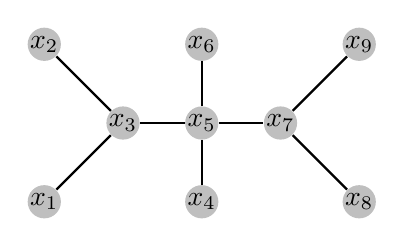
\begin{tikzpicture}[scale=1]
    % Draw a 7,11 network
    % First we draw the vertices
    \foreach \pos/\name in {{(1,1)/x_1}, {(1,3)/x_2}, {(2,2)/x_3}, {(3,1)/x_4}, {(3,2)/x_5}, {(3,3)/x_6}, {(4,2)/x_7}, {(5,1)/x_8}, {(5,3)/x_9}}
        \node[vertex] (\name) at \pos {$\name$};
    
    
    % Connect vertices with edges 
    \foreach \source/ \dest in {x_1/x_3, x_2/x_3,x_3/x_5,x_4/x_5, x_6/x_5, x_5/x_7, x_7/x_8, x_7/x_9}
        \path[edge] (\source) -- (\dest) ;
        
\end{tikzpicture}

\end{center}



\begin{center}
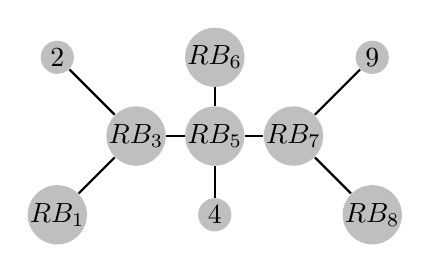
\begin{tikzpicture}[scale=1]
    % Draw a 7,11 network
    % First we draw the vertices
    \foreach \pos/\name in {{(1,1)/RB_1}, {(1,3)/2}, {(2,2)/RB_3}, {(3,1)/4}, {(3,2)/RB_5}, {(3,3)/RB_6}, {(4,2)/RB_7}, {(5,1)/RB_8}, {(5,3)/9}}
        \node[vertex] (\name) at \pos {$\name$};
    
    
    % Connect vertices with edges 
    \foreach \source/ \dest in {RB_1/RB_3, 2/RB_3,RB_3/RB_5,4/RB_5, RB_6/RB_5, RB_5/RB_7, RB_7/RB_8, RB_7/9}
        \path[edge] (\source) -- (\dest) ;
        
\end{tikzpicture}
\end{center}

Assume $X_{I^0_3}>X_{I^0_5}$ and $X_{I^0_7}>X_{I^0_5}$. Since that, Rebel 5 will get the information from Rebel 3,7 before he reports $I^0_5$. Since that, Rebel 5 has a profitable deviation by just reporting $\bar{I}^0_5=x_3\times x_5\times x_7<I^0_5$ to let Rebel 3 and Rebel 7 think he is still in the path and initiating the coordination to \textbf{revolt}. Rebel 6 can detect such deviation since $\bar{I}^0_5$ did not include Rebel 6's own index $x_6$. However, if Rebel 6 forms the off-path belief as Equation ~\ref{eq_grim_trigger}, he will then play \textbf{stay} forever although the coordination to \textbf{revolt} has been initiated.

\end{example}

Due to the pay-off function is not strictly increasing with the number of \textbf{revolts}, some Rebels will be excluded from coordination with this grim-trigger-like off-path belief. As Example ~\ref{ex_deviation} shows, some strategies other than $I^t$ have to be considered as the strategies in the equilibrium path to avoid the situation where some Rebels are out of an existing coordination. The introducing of message $\langle 1 \rangle$ gives more equilibrium paths when grim trigger is adopted. 

\subsubsection{Sketch of the proof for Theorem ~\ref{thm_main_result}}

In previous subsections, I have listed the belief updating in equilibrium path by showing the the belief updating after observing various messages. Lemma ~\ref{lemma_in_the_path} shows that such equilibrium path is APEX . 
\begin{lemma}\label{lemma_in_the_path}
If the state has strong connectedness, then for all $n$-person repeated $k$-Threshold game with parameter $1\leq k\leq n$ played in any FFCCU network without cycles, there is an APEX path.
\end{lemma}

For the histories outside of equilibrium path, they could be detectable or undetectable. The argument to prove Theorem ~\ref{thm_main_result} is as follows. First, I use off-path belief to prevent players from making detectable deviations, such as deviations from playing the specified forms of sequences listed in Table ~\ref{Table_msg_reporting} and ~\ref{Table_msg_coordination}. Then I argue that any undetectable deviation made by a Rebel before he knows the relevant information, $\#[Rebels](\theta)\geq k$ or $\#[Rebels](\theta)< k$, will create noises in his own learning process and then reduce his own expected continuation pay-off.  To see why making undetectable deviation will create noises to impede the learning process before he knows the relevant information, consider the case when a Rebel wants to mimic pivotal plays' behaviors by sending $\langle 1 \rangle$. According to Table ~\ref{Table_blf_up_cdt11} and Table ~\ref{Table_blf_up_cdt12}, the continuation playing by his neighbors after observing $\langle 1 \rangle$ is to play \textbf{stay} forever or to play \textbf{revolt} forever. Since all his neighbors repeats the same action, he can not learn additional information about $\theta$. When $\delta$ is high enough, since he can learn the relevant information by Lemma ~\ref{lemma_learn} if he stays in the path, he is better off by staying in the equilibrium path to achieve the maximum static pay-off as 1 when $\#[Rebels](\theta)\geq k$ and achieve the maximum static pay-off as 0 when $\#[Rebels](\theta)< k$. Claim ~\ref{claim_can_not_pretend_almost_success} shows this argument.

\subsection{Discussion}
\label{sec:varies}


\subsubsection{Variation: Pay-off as signals}
The assumption on the observability of pay-off can be relaxed without changing the result in Theorem ~\ref{thm_main_result}. One may consider a situation in which the static pay-off depends not only on joint efforts but also depends on other random effects, say the weather.\footnote{e.g.,\citep{SHADMEHR2011}}. Specifically, let's suppose that Rebels' actions can generate a public signal $y\in \{y_1,y_2\}$. Denote Rebel $i$'s pay-off function by $u_{Rebel}(a_{Rebel_i},y)$, and let $u_{Rebel}(\textbf{stay},y_1)=u_{Rebel}(\textbf{stay},y_2)=u_0$. The distribution of $y_1$ and $y_2$ is as the following.
\begin{eqnarray*}
p_{1s} &=& \mathrm {Pr}(y=y_1|\#\textbf{revolt}\geq k) \\
p_{1f} &=& \mathrm {Pr}(y=y_1|\#\textbf{revolt}< k) \\
p_{2s} &=& \mathrm {Pr}(y=y_2|\#\textbf{revolt}\geq k) \\
p_{2f} &=& \mathrm {Pr}(y=y_2|\#\textbf{revolt}< k) 
\end{eqnarray*}
. Moreover, let's suppose
\begin{equation}
p_{1s}u_{Rebel}(\textbf{revolt}, y_1)+p_{2s}u_{Rebel}(\textbf{revolt}, y_2)>u_0>p_{1f}u_{Rebel}(\textbf{revolt}, y_1)+p_{2f}u_{Rebel}(\textbf{revolt}, y_2)
\end{equation}
and
\begin{equation}
1>p_{1s}>0,1>p_{2s}>0,p_{1f}=1-p_{1s},p_{2f}=1-p_{2s}
\end{equation}

Equation (6) is a generalization for the previous setting. Equation (7) is a full support assumption on signal $y$. 

We can construct exactly the same equilibrium strategies by ignoring the noisy signal $y$ when Equation (7) holds. By directly checking the equilibrium path constructed in previous sections (see also Table ~\ref{Table_msg_reporting} and ~\ref{Table_msg_coordination}), \textit{at most one} Rebel playing \textbf{revolt} in a period before some Rebels play $\langle 1 \rangle$, and thus the signal $y$ is not relevant before some Rebels play $\langle 1 \rangle$. Moreover, playing $\langle 1 \rangle$ comes from a Rebel's observation in reporting period where Rebels' strategies are independent from $y$, and thus playing $\langle 1 \rangle$ is independent from $y$. We then just check if a Rebel wants to deviate to play $\langle 1 \rangle$. According to equilibrium strategies in the path, however, playing $\langle 1 \rangle$ will incur either coordination to \textbf{stay} or coordination to \textbf{revolt} after current block as Table ~\ref{Table_blf_up_cdt11} and Table ~\ref{Table_blf_up_cdt12} shows. Since signal $y$ is noisy, and since Rebels' actions will repeat, he can not learn the relevant information. As the same argument in Claim ~\ref{claim_can_not_pretend_almost_success}, he is better off by staying in the equilibrium path.

If Equation (7) fails, and so that the signal $y$ is not noisy, says $p_{1s}=p_{2f}=1$, the equilibrium constructed in the previous section is no longer an equilibrium. However, another APEX equilibrium can be constructed by letting all Rebels play \textbf{revolt} in the first period, and then keep playing \textbf{revolt} or \textbf{stay} contingent on the signals $y=y_1$ or $y=y_2$ when $\delta$ is sufficiently high.

\subsubsection{Variation: Rebels with different levels of efforts}

Consider a model in which players have different levels of efforts contributing to a collective action. Denote the set of states of nature by $\hat{\Theta}=\Theta \times \Xi$, where $\Xi=\{1,2,...,k\}^n$. Let $\hat{\theta}=(\theta,e)$, where $\theta\in \Theta$ and $e\in \Xi$. $\hat{\theta}$ is interpreted as a state of nature in which a player $i$ could be either a Rebel or Inert with $e_i$ efforts, where $e_i\in \{1,2,...,k\}$. When a Rebel $i$ plays \textbf{revolt}, he contributes $e_i$ efforts to a collective action, while the success of such collective action requires $k$ amount of efforts. If the collective action succeed, such Rebel $i$ will get $b_i>0$ as his reward. The pay-off structure is modified as the following.
\begin{enumerate}
\item $u_{Rebel_i}(a_{Rebel_i},a_{-\theta_i})=b_i$ if $a_{Rebel_i}=\textbf{revolt}$ and $\sum_{j:a_{\theta_j}=\textbf{revolt}}e_j\geq k$
\item $u_{Rebel_i}(a_{Rebel_i},a_{-\theta_i})=-e_i$ if $a_{Rebel_i}=\textbf{revolt}$ and $\sum_{j:a_{\theta_j}=\textbf{revolt}}e_j< k$
\item $u_{Rebel_i}(a_{Rebel_i},a_{-\theta_i})=0$ if $a_{Rebel_i}=\textbf{stay}$
\item $u_{Inert_i}(a_{Inert_i},a_{-\theta_i})=1$ if $a_{Inert_i}=\textbf{stay}$
\end{enumerate}

After the nature chooses a $\hat{\theta}$, players play the above game in a network $G$ infinitely repeatedly. To see that the equilibrium constructed in previous section is still an equilibrium, let's transform the network and the state $(G,\hat{\theta})$ to $(G^{'},\hat{\theta}^{'})$ in which, there are $e_i$ different players attached to a single player $i$ for each $i\in N$, and all the players have levels of efforts as 1. What matters here is that the states of nature are finite and discrete, and therefore we can use prime indexing to construct an equilibrium .


\subsubsection{Variation: networks with cycles}

The prime indexing can deal with a potential free problem in cyclic networks, although we may need to redefine the information hierarchy in order to redefine which Rebels are needed to report their private information in the equilibrium. Let's consider the following Example ~\ref{ex_no_free_rider_cycle}.

\begin{example}
\label{ex_no_free_rider_cycle}
Let $k=6$. Rebel 3 and Rebel 4 have the same information $I^1_3=I^1_4$. Since reporting is costly, if there is no punishment, Rebel 3 (resp. Rebel 4) may shirk and deviate from truthfully reporting if Rebel 4 (resp. Rebel 3) reports truthfully. However, this kind of deviation can be detected by Rebel 5 (or Rebel 2) since $I^1_3$ should be equal to $I^1_4$. 

\begin{center}
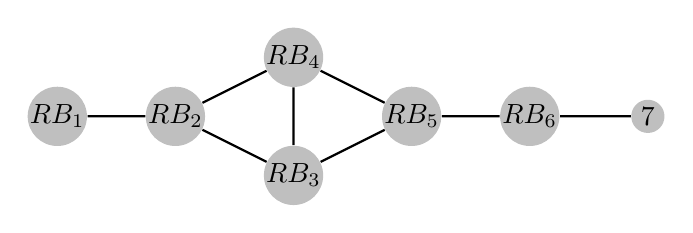
\begin{tikzpicture}[scale=1.5]
    % Draw a 7,11 network
    % First we draw the vertices
    \foreach \pos/\name in {{(1,2)/RB_1}, {(2,2)/RB_2}, {(3,1.5)/RB_3}, {(3,2.5)/RB_4}, {(4,2)/RB_5}, {(5,2)/RB_6}, {(6,2)/7}}
        \node[vertex] (\name) at \pos {$\name$};
    
    
    % Connect vertices with edges 
    \foreach \source/ \dest in {RB_1/RB_2, RB_2/RB_3,RB_2/RB_4,RB_3/RB_5, RB_4/RB_5, RB_5/RB_6, 7/RB_6, RB_4/RB_3}
        \path[edge] (\source) -- (\dest) ;
        
\end{tikzpicture}
\end{center}

\end{example}

Indeed, this monitoring technique will be less invalid if the network is not commonly known. In this example, if Rebels has asymmetric information about network structure, says Rebel 5 (or Rebel 2,3) does not certain about if there is a link between Rebel 4 and Rebel 2, then Rebel 4 can just pretend that he doesn't know Rebel 2\footnote{However, if there is asymmetric information about network structure, then Example ~\ref{ex_no_free_rider_cycle} is not exactly a free rider problem. Dependent on what asymmetric information is given, Rebel 3 and Rebel 4 then have different incentives in untruthful reporting. Untruthful reporting could be a dominant strategy for Rebel 4 but not necessary be a dominant strategy for Rebel 3.}. The analysis in incomplete information about network structure is beyond the scope of this paper. Recent papers such as \citep{Galeotti2010} deal with the issues when the network is not commonly known.

There is another free rider problem which is harder to deal with. Recall that the implicit technique in my equilibrium construction is that a free rider can be selected before the game enters at each reporting period in each block. When the networks has cycles, the selection of free rider needs more elaboration. Let's consider Example ~\ref{ex_free_rider_cycle}.
\begin{example}\label{ex_free_rider_cycle}
Let $k=6$. Suppose the network and $\theta$ is as the following. 

\begin{center}
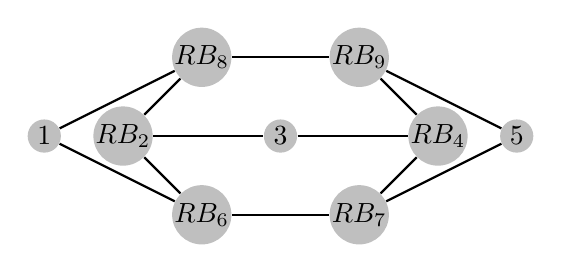
\begin{tikzpicture}[scale=1]
    % Draw a 7,11 network
    % First we draw the vertices
    \foreach \pos/\name in {{(1,3)/1}, {(2,3)/RB_2}, {(4,3)/3}, {(6,3)/RB_4}, {(7,3)/5}, {(3,2)/RB_6}, {(5,2)/RB_7}, {(3,4)/RB_8}, {(5,4)/RB_9}}
        \node[vertex] (\name) at \pos {$\name$};
    
    
    % Connect vertices with edges 
    \foreach \source/ \dest in { 1/RB_6, 1/RB_8, RB_2/3, RB_2/RB_8, 3/RB_4, RB_2/RB_6, RB_6/RB_7, RB_8/RB_9, RB_9/RB_4, RB_7/RB_4, RB_9/5, RB_7/5}
        \path[edge] (\source) -- (\dest) ;
        
\end{tikzpicture}
\end{center}

Assume that one round of reporting is done. Rebel 2 has known $\{RB_2,RB_6,RB_8,RB_9,RB_7\}$, Rebel 4 has known $\{RB_4,RB_7,RB_9,RB_8,RB_6\}$, and so on. One more round of reporting will let Rebels 3,6,7,4,9,8 know the true state $\theta$, and therefore Rebels 3,6,7,4,9,8 are all pivotal players. We may have a rule as Example ~\ref{ex_free_rider_tree} to pick up a free rider. For instance, we pick Rebel 4 before the game entering at the next reporting period. However, this free-rider selection is ex-post. The true state $\theta^{'}$ could be the following.

\begin{center}
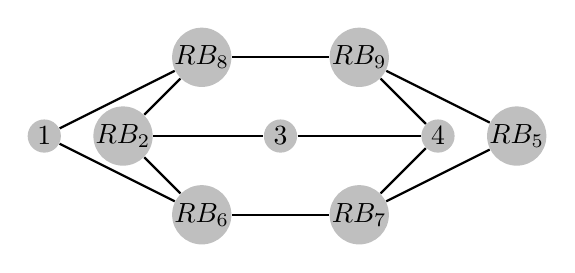
\begin{tikzpicture}[scale=1]
    % Draw a 7,11 network
    % First we draw the vertices
    \foreach \pos/\name in {{(1,3)/1}, {(2,3)/RB_2}, {(4,3)/3}, {(6,3)/4}, {(7,3)/RB_5}, {(3,2)/RB_6}, {(5,2)/RB_7}, {(3,4)/RB_8}, {(5,4)/RB_9}}
        \node[vertex] (\name) at \pos {$\name$};
    
    
    % Connect vertices with edges 
    \foreach \source/ \dest in { 1/RB_6, 1/RB_8, RB_2/3, RB_2/RB_8, 3/4, RB_2/RB_6, RB_6/RB_7, RB_8/RB_9, RB_9/4, RB_7/4, RB_9/RB_5, RB_7/RB_5}
        \path[edge] (\source) -- (\dest) ;
        
\end{tikzpicture}
\end{center}

Now node 4 is an Inert and so that he is not a pivotal Rebel. A selection rule has to be applied to select a pivotal Rebel (say, Rebel 5) during the game played in reporting period. 

\end{example}

As Example ~\ref{ex_free_rider_tree} or ~\ref{ex_free_rider_cycle} show, a free rider problem may occur if a free rider has not been selected before the game enters at the reporting period. In cyclic networks, this problem seems more severe and a free-rider selection is needed. Though it is possible to construct a selection rule, this rule is still infeasible in this paper. 

I leave a conjecture here and end this section.

\begin{conjecture}
For $n$-person repeated $k$-Threshold game with parameter $1\leq k < n$ played in any FFCCU network,
if the $\pi$ has full support on strong connectedness, then there is a $\delta^{*}$ such that a (weak) APEX sequential equilibrium exists whenever $\delta\in(\delta^{*},1)$.
\end{conjecture}



\section{Conclusion}
\label{sec:con}

I answer how various types of networks can serve to induce collective action by modeling a coordination game and illustrating the learning process generated by strategies in a sequential equilibrium. In the equilibrium, players transmit relevant information by encoding such information through their actions in the time horizontal line. Since an expected cost exists in coding information, free rider problems may occur and impede the learning process. When the networks are FFCCU without cycle, players can always learn the underlying relevant information and coordinate only through their actions. However, the kinds of equilibrium strategies that can constitute a learning process for obtaining relevant information in cyclic networks still remains unanswered.

The construction of communication protocol exploits the assumption of finite type space and the finite threshold. Since relevant information has been parameterized as a threshold, players can acquire this information by gradually reporting their own private information. The major punishment to keep players in the equilibrium path is then the shift through coordination to play the same actions terminating new updates on their information. The threshold model seems to be a general model for proving that a communication protocol  does not only lead to a learning process but also constitutes an equilibrium revealing relevant information in finite time.


Existing literature in political science and sociology have recognized the importance of social networks in influencing individuals' participation in social movements, e.g., \citep{Passy2003}\citep{McAdam2003}\citep{Siegel2009}. This paper views networks as routes for communication where rational individuals initially have local information and can influence nearby individuals by taking actions. Such influence may take a long time to travel across individuals. The whole process incurs inefficient outcomes in many periods. Although characterization in the speed of information transmission across a network is not answered here, it is an important topic for raising more attentions to investigate the most efficient way to spread information . This question would remain for the future research.




\bibliographystyle{abbrvnat}	% (uses file "plain.bst")
\bibliography{jmp_ref}		% expects file "myrefs.bib"


\appendix
\section{Appendix}

\noindent\textbf{proof for Lemma ~\ref{lemma_learn}}

\begin{proof}
The proof is done by contradiction. Suppose Rebels' strategies constitute an APEX. By definition of APEX, there is a time $T^{\theta}$ when actions start to repeat at state $\theta$. Let $T=\max_{\theta\in \Theta}{T^{\theta}}$. Pick that time $T_i=T+1$ and suppose the consequence did not not holds so that $0<\sum_{\theta:\#[Rebels](\theta)\geq k}\beta^{\pi,\tau^*}_{G_i}(\theta|h^{s}_{G_i})<1$ for some $s\geq T_i$. Then this Rebel puts some positive weights on some $\theta\in \{\theta:\#[Rebels](\theta)< k\}$ and puts some positive weights on $\theta\in \{\theta:\#[Rebels](\theta)\geq k\}$ at that time $s$. Note this Rebel $i$ has already known $\theta_j$ if $j\in G_i$, and therefore Rebel $i$ put some positive weights on $\theta\in \{\theta:\#[Rebels](\theta)< k, \theta_l=Rebel, l\notin G_i\}$ and $\theta\in \{\theta:\#[Rebels](\theta)< k, \theta_l=Inert, l\notin G_i\}$. Since actions start to repeat at $T$, all $i$'s neighbors will play the same actions as the actions at time $T$, but then Rebel $i$ can not update information from his neighborhood by Bayesian rule. Suppose $i$'s continuation strategy is to play \textbf{revolt} repeatedly, then this is not ex-post efficient if $\#[Rebels](\theta)< k$. Suppose $i$'s continuation strategy is to play \textbf{stay} repeatedly, then this is not ex-post efficient if $\#[Rebels](\theta)\geq k$
\end{proof}

\bigskip
\noindent\textbf{proof for Theorem ~\ref{lemma_empty}}

This proof follows three useful claims, Claim ~\ref{lemma_I_subset_N}, Claim ~\ref{lemma1} and Claim ~\ref{lemma_connected}. First note that $I^t_i$ and $N^t_i$, $t\geq 1$ can be expressed as 
\begin{equation}
\label{eq_info_nb}
I^{t}_i = \bigcup_{k_0\in G_i\cap R^{t}}\bigcup_{k_1\in G_{k_0}\cap R^{t-1}}...\bigcup_{k_{t-1}\in G_{k_{t-2}}\cap R^{1}}G_{k_{t-1}}\cap R^0
\end{equation}
, while $H^t_i$ can be expressed as
\begin{equation}
\label{eq_nb}
N^t_i = \bigcup_{k_0\in G_i\cap R^{t-1}}\bigcup_{k_1\in G_{k_0}\cap R^{t-2}}...\bigcup_{k_{t-2}\in G_{k_{t-3}}\cap R^{0}}G_{k_{t-2}}
\end{equation}

\begin{claim}
\label{lemma_I_subset_N}
$I^t_i\subset N^t_i$ for $t\geq 1$
\end{claim}
\begin{proof}
$I^t_0\subset N^t_0$ by definition. Since $R^t\subset R^{t-1}$ for $t\geq 1$, $I^t_i\subset N^t_i$ for $t\geq 1$ by comparing Equation ~\ref{eq_info_nb} and Equation ~\ref{eq_nb}.
\end{proof}

\begin{claim}
\label{lemma1}
If the network is FFCCU without cycle, then for each $t\geq 1$ block, we have $i\in R^t\Leftrightarrow i\in R^{t-1} \text{ and } \exists k_1,k_2\in R^{t-1}\cap \bar{G}_i$, where $k_1\neq k_2$.
\end{claim}
\begin{proof}
The proof is by induction. We first show that the statement is true for $t=1$. 

\textbf{Base}: $i\in R^1\Leftrightarrow [i\in R^0] \wedge [\exists k_1,k_2\in (R^0\cap \bar{G}_i)]$. 

$\Rightarrow$: Since $i\in R^1$, then $i\in R^0$ and then $I^0_i\nsubseteq N^0_j$ for all $j\in \bar{G}_i$ by definition. Since $I^0_i=R^0\cap G_i$, then $\forall j\in \bar{G}_i [\exists k\in (R^0\cap \bar{G}_i) [k\notin N^0_j]]$. Since the $j\in \bar{G}_i$ is arbitrary,  we then have a pair of $k_1, k_2 \in (R^0\cap \bar{G}_i)$ such that $k_1\notin N^0_{k_2}$ and $k_2\notin N^0_{k_1}$.

$\Leftarrow$: Pick $k\in \{k_1,k_2\}\subseteq (R^0\cap \bar{G}_i)$, and pick an arbitrary $j\in \bar{G}_i\backslash \{k\}$. Note that $k\notin N^0_j$, otherwise there is a cycle from $i$ to $i$. Hence $[k\in (R^0\cap \bar{G}_i)] \wedge [k\notin N^0_j]$ and therefore $[k\in I^0_i] \wedge [k\notin N^0_j]$. Then we have $I^0_i\nsubseteq N^0_j$ for arbitrary $j\in \bar{G}_i$, and thus $i\in R^1$.

\textbf{Induction hypothesis}: the statement is true for $\{1,2,..,t\}$ where $t\geq 1$. 


If the hypothesis is true, then $i\in R^{t+1}\Leftrightarrow [i\in R^{t}] \wedge [\exists k_1,k_2\in (R^{t}\cap \bar{G}_i)]$


$\Rightarrow$: since $i\in R^{t+1}$, then $i\in R^t$ and $I^t_i\nsubseteq N^t_j$ for all $j\in \bar{G}_i$ by definition. Recall that $I^t_i$ can be expressed as Equation ~\ref{eq_info_nb} and $H^t_i$ can be expressed as Equation ~\ref{eq_nb}, then for every $l\in I^{t-1}_i$, we can find a path connecting $i$ to $l$ by the induction hypothesis. If $j\in \bar{G}_i$, then we can find a path connecting $j$ to $l$ by connecting $j$ to $i$, and then connecting $i$ to $l$. Thus, if $l\in I^{t-1}_i$ then $l\in N^t_J$, and hence $I^{t-1}_i\subseteq N^t_{j}$ for all $j\in \bar{G}_i$. Recall that $I^t_i = \bigcup_{k\in N_i\cap R^t}I^{t-1}_k$ and $i\in R^{t+1}$, then we must have $\forall j\in \bar{G}_i [\exists k\in (R^t\cap \bar{G}_i)[ I^{t-1}_k\nsubseteq N^t_j]]$, since $I^{t-1}_i\subseteq N^t_{j}$. Note that such $j\in \bar{G}_i$ is arbitrary,  we then have a pair of $k_1, k_2 \in (R^{t}\cap \bar{G}_i)$ such that $k_1\notin N^t_{k_2}$ and $k_2\notin N^t_{k_1}$.
\bigskip

$\Leftarrow$:
By the induction hypothesis, we have a chain $k_{1_0},...,k_{1_t},i,k_{2_t},...,k_{2_0}$ with $k_{1_0}\in R^0$,..., $k_{1_t}\in R^t$, $i\in R^t$, $k_{2_t}\in R^t$,...,$k_{1_0}\in R^0$, where $k_{1_t},k_{2_t}\in (R^{t}\cap \bar{G}_i)$, $k_{1_0}\in I^{t-1}_{k_{1_t}}$ and $k_{2_0}\in I^{t-1}_{k_{2_t}}$. Note that $k_{1_0}\notin N^t_j$ whenever $j\in \bar{G}_i$, otherwise there is a cycle from $i$ to $i$ since $\{i,k_{2_t},...,k_{2_0}\}\in N^t_j$, and hence $[k_{1_0}\in I^{t-1}_{k_{1_t}}] \wedge [k_{1_0}\notin N^t_j]$ for all $j\in \bar{G}_i$. Therefore we have $[I^{t-1}_{k_{1_t}}\in I^t_i] \wedge [I^{t-1}_{k_{1_t}}\notin N^t_j]$ for all $j\in \bar{G}_i$ since $k_{1_t},k_{2_t}\in (R^{t}\cap \bar{G}_i)$ and $[k_{1_0}\in I^{t-1}_{k_{1_t}}] \wedge [k_{1_0}\notin N^t_j]$ for all $j\in \bar{G}_i$. Then we have $I^t_i=\bigcup_{k\in N_i\cap R^{t}}I^{t-1}_k\nsubseteq N^t_j$ for arbitrary $j\in \bar{G}_i$, and thus $i\in R^{t+1}$.



We can then conclude that the statement is true by induction.




\end{proof}



\begin{claim}
\label{lemma_connected}
If the network FFCCU without cycle and if the state has strong connectedness, then if there is a pair of $R^{t}$ nodes then there exists a $R^{t}$-path connecting them.
\end{claim}
\begin{proof}
The proof is by induction and by Claim ~\ref{lemma1}. Since the state has strong connectedness, we have a $R^0$-path connecting each pair of $R^0$ nodes. Since all pairs of $R^0$ nodes are connected by a $R^0$-path, then for all pairs of $R^1$ nodes must be in some of such paths by Claim ~\ref{lemma1}, and then connected by a $R^0$-path. But then all the $R^0$-nodes in such path are all $R^1$ nodes by Claim ~\ref{lemma1} again and by $R^t\subseteq R^{t-1}$ for $t\geq 1$ by definition. Thus, for all pairs of $R^1$ nodes has a $R^1$-path connecting them. The similar argument holds for $t> 1$, we then get the result.

\end{proof}
I begin to prove this Theorem ~\ref{lemma_empty}. I first claim that if $R^t\neq \emptyset$ and if $R^{t+1}= \emptyset$, then $R^0\subset I^t_i$ whenever $i\in R^t$. Then I claim that if $R^t\neq \emptyset$ then $\# R^{t+1}<\# R^t$. Finally, I iterate $R^t$ with $t\geq 0$ to get the conclusion.

If $R^t\neq \emptyset$ but $R^{t+1}= \emptyset$, I claim that $R^0\subset I^{t}_i$ for all $i\in R^t$. The proof is by contradiction. If $R^0\not\subset I^{t}_i$, there is a $j\in R^0$ but $j\notin I^t_i$. Since $I^t_i$ can be expressed as Equation ~\ref{eq_info_nb}, there is no such a path $\{i,k_0,k_1,...,k_{t-1},j\}$, where $k_0\in G_i\cap R^{t},k_1\in G_{k_0}\cap R^{t-1},...,k_{t-1}\in N_{k_{t-2}}\cap R^{1}$. Since $R^{t+1}=\emptyset$ and therefore $R^{t^{'}}=\emptyset$ if $t^{'}\geq t+1$, and hence there is no such a path containing a node in $R^{t^{'}}=\emptyset$, where $t^{'}\geq t+1$ connecting $i$ to $j$. But $i\in R^t$ and $i,j\in R^0$, if there is no such a path, then it violate either Claim ~\ref{lemma_connected} or Claim ~\ref{lemma1}. Contradiction.

Next I claim that if $R^t\neq \emptyset$ then $\# R^{t+1}<\# R^t$. The proof is the followings. Given a node $i$ in $R^t$, let $j\in R^t$ (could be $i$ itself) be the node connected with $i$ with the maximum shortest $R^t$ path. This $j$ can be found since $R^t\neq \emptyset$ and the network is finite. Then there is no $R^t$ node in $j$'s neighborhood other than the nodes in this path. Since the network is without cycle, there is at most one $R^t$ node in $j$'s neighborhood. But then $j\notin R^{t+1}$ since it violate Claim ~\ref{lemma1}.

Starting from $R^0\neq \emptyset$ and iterating $R^t$ with $t\geq 0$, if $R^t\neq \emptyset$ but $R^{t+1}= \emptyset$, then there is some $i$ with $R^0\subset I^t_i$ as the above paragraph shows; if $R^t\neq \emptyset$ and $R^{t+1}\neq \emptyset$, then we starting from $R^{t+1}$ and iterating $R^{t+1}$ with $t\geq t+1$. Since $\#R^{t+1}<\#R^t$ as the above paragraph shows, there is a time $t^{*}$ with $R^{t^{*}}=\emptyset$, then we get the conclusion.


\bigskip




\noindent\textbf{proof for Lemma ~\ref{lemma_at_most_two_nodes}}

\begin{proof}
Denote $(i,j)$-path as the set of paths from $i$ to $j$. The proof is by contradiction. Suppose there are three or more $R^t$-nodes in $C^t$, then pick any three nodes of them, and denote them as $i_1,i_2,i_3$. Let's say $i_2$ is in a $(i_1,i_3)$-path by strong connectedness, and therefore $i_2\in Tr_{i_1i_2}$ and $i_3\in Tr_{i_2i_3}$. First we show that $i_1\in G_{i_2}$ (or $i_3\in G_{i_2}$). Suppose $i_1\notin N_{i_2}$, since $i_1,i_2\in R^t$, then the $(i_1,i_2)$-path is a $R^t$-path by Claim ~\ref{lemma1}. Let this $(i_1i_2)$-path be $\{i_1,j_1,...,j_n,i_2\}$. Since $i_1,j_1,...,j_n,i_2\in R^t$, we then have $I^{t-1}_{i_1}\nsubseteq N^{t-1}_{j_1},...,I^{t-1}_{j_n}\nsubseteq N^{t-1}_{i_2}$ and $I^{t-1}_{j_1}\nsubseteq N^{t-1}_{i_1},...,I^{t-1}_{i_2}\nsubseteq N^{t-1}_{j_n}$. Since $I^{t-1}_{i_1}\subseteq N^{t-1}_{i_1},...,I^{t-1}_{i_2}\subseteq N^{t-1}_{i_2}$ by Claim ~\ref{lemma_I_subset_N}, we further have $\exists k_1\in R^0[k_1\in N^{t-1}_{j_1}\backslash I^{t-1}_{i_1}]$,...,$\exists k_n\in R^0[k_n\in N^{t-1}_{j_n}\backslash I^{t-1}_{i_2}]$. Since the state has strong connectedness, there is a $R^0$ path connecting $k_1,...,k_n$ by Claim ~\ref{lemma_connected}. But then we have already found $k_1,k_2$ such that $k_1\in N^{t-1}_{j_1}\backslash I^{t-1}_{i_1}$ and $k_2\in \bar{G}_{k_1}$. It is a contradiction that $i_1\in C$.

Now, $i_1,i_2,i_3$ will form a $R^t$-path as $\{i_1,i_2,i_3\}$. With the same argument as the above, we then have $\exists k_1\in R^0[k_1\in N^{t-1}_{i_2}\backslash I^{t-1}_{i_1}]$ and $\exists k_2\in R^0[k_2\in N^{t-1}_{i_3}\backslash I^{t-1}_{i_2}]$, and thus $i_1$ is not in $C$.
\end{proof}


\noindent\textbf{proof for Lemma ~\ref{lemma_no_node_outside}}
\begin{proof}
The proof is done by contradiction. Since $i\in R^t$, there is a $j\in (R^{t-1}\cap \bar{G}_i)$ by Lemma ~\ref{lemma1}. Note that $N^{t-1}_j\subseteq \bigcup_{k\in N^{t-1}_i}N_k$ since $N^{t-1}_j =\bigcup_{k\in I^{t-2}_j}N_k$, and $I^{t-2}_j\subseteq I^{t-1}_i\subseteq N^{t-1}_i$. If there is another node outside $\bigcup_{k\in N^{t-1}_i}N_k$ in $Tr_{ij}$, then there must be another node such that there is a path connected to some nodes in $N^{t-1}_j$ since the network is connected. It is a contradiction that $i\in C$.

\end{proof}

\subsection{Equilibrium}
\label{Apn_equilibrium}
\subsubsection{Off-path belief}

If Rebel $i$ detects a deviation at $m$ period, he form the belief as
\begin{equation}
\beta_{i}(\{\theta:\theta\in \times_{j\in G_i}\{\theta_j\}\times\{Inert\}^{n-\#G_i}\}|h^{m^{'}}_{G_i})=1 \text{ , } m^{'}\geq m
\end{equation}



\subsubsection{Equilibrium Path: Notations}


\begin{itemize}

\item $\langle \rangle_r$ be the set of finite sequences in which the action \textbf{r} occurs once and only once.
\item $PF(\langle \rangle,m)$ be the $m$-periods prefix of a finite sequence $\langle \rangle$.
\item $(i,j)$-path be the set of paths from $i$ to $j$.

\end{itemize}

\subsubsection{Equilibrium Path: reporting period}

\paragraph{reporting period: notations}
\begin{itemize}
\item $m$ be a period in reporting period in $t$ block.
\item $|\langle RP^t \rangle|$ be the total periods in reporting period in $t$-block
\item $O^{m,t}_i$ be the set of $i$'s neighbors $j$s who has played a sequence $M$ such that $M=PF(\langle I^{t-1}_j \rangle,m)$ and $M \in \langle \rangle_r$ at period $m$. 
\item $I^{m,t}_i\equiv (\bigcup_{k\in O^{m,t}_i} I^{t-1}_k)\cup I^{t-1}_i$ be the updated relevant information gathered by $i$ at period $m$. Note that $I^{0,t}_i=I^{t-1}_i$ and $I^{|\langle RP^t \rangle|,t }_i=I^{t}_i$.
\item $N^{m,t}_i\equiv (\bigcup_{k\in O^{m,t}_i} N^{t-1}_k)\cup N^{t-1}_i$
be the updated neighborhood which contains $I^{m,t}_i$

\item Let 
\[Ex_{I^{m,t}_i}\equiv \{l\notin N^{m,t}_i|\exists l^{'}\in I^{m,t}_i\text{ such that there exists a $(l,l^{'})$-path}\}\]
be all the possible Rebel nodes outside of $N^{m,t}_i$ given $I^{m,t}_i$
\item Let
\[Tr_{I^{m,t}_ij}\equiv Tr_{ij}\cap (Ex_{I^{m,t}_i}\cup I^{m,t}_i)\]
be all the possible Rebel nodes in the $Tr_{ij}$ given $I^{m,t}_i$. 
\end{itemize}
\paragraph{reporting period: automata}

The equilibrium path in the reporting period is presented by an automata. In this automata, there are six sub-automatas: WHILE LOOP, MAIN, CHECK.$0$, CHECK.$m$, CHECK.$k$, and POST-CHECK. In the beginning of reporting period (at $m=0$), each player plays the game according to the description in WHILE LOOP. Then, each player follows the description of a sub-automata if he were running that sub-automata.

\subparagraph{$i\notin R^{t}$}




\begin{itemize}
\item \textbf{WHILE LOOP}
\begin{itemize}
\item At $m\geq 0$, if $\#Ex_{I^{m,t}_i}\cup I^{m,t}_i< k$, report $\langle \textbf{stay} \rangle$ and then play \textbf{stay} forever.
\item Otherwise, runs \textbf{POST-CHECK }
\end{itemize}
\end{itemize}

\subparagraph{$i\in R^{t}$}

\begin{itemize}

\item \textbf{WHILE LOOP}
\begin{itemize}
\item At $m\geq 0$, if $\# Ex_{I^{m,t}_i}\cup I^{m,t}_i< k$, report $\langle \textbf{stay} \rangle$ and then play \textbf{stay} forever.
\item Otherwise, runs \textbf{MAIN }
\end{itemize}


\item \textbf{MAIN}

At $m\geq 0$, 

\begin{enumerate}
\item At $m=0$ and if $\# I^{t-1}_i=\# I^{0,t}_i= k-1$, then 
runs \textbf{POST-CHECK }


\item At $m=0$ and if $i\in R^t$ and
\[\nexists j\in R^{t-1}\cap\bar{G}_i \text{ such that }\exists l_1,l_2\in Tr_{ij}[[l_1\in N^{t-1}_j\backslash I^{t-1}_i] \wedge [l_2\in \bar{G}_{l_1}]]\]
, then runs \textbf{CHECK.$0$}. Otherwise, recall \textbf{MAIN}
\item At $0\leq m \leq |RP^t|-|\langle I^{t-1}_i \rangle|$, play
\[\textbf{stay}\]
\item At $m = |RP^t|-|\langle I^{t-1}_i \rangle|+1$, then
\begin{enumerate}
\item if $O^{m,t}_i= \emptyset$ 
, then report
\[\langle I^{t-1}_i \rangle\]
\item if $O^{m,t}_i\neq \emptyset$, then runs \textbf{CHECK.k}

\end{enumerate}

\end{enumerate}





\item \textbf{CHECK.$0$}

At $m=0$, if $i\in C^t$, i.e. if $i\in R^t$ and
\[\nexists j\in R^{t-1}\cap \bar{G}_i \text{ such that }\exists l_1,l_2\in Tr_{ij}[[l_1\in N^{t-1}_j\setminus I^{t-1}_i] \wedge [l_2\in \bar{G}_{l_1}]]\]
, then
\begin{enumerate}
\item If $\#C^t=1$
, then runs
\textbf{POST-CHECK }

\item If $\#C^t=2$, then denote $i_1,i_2\in C$ such that $I^{t-2}_{i_1}<I^{t-2}_{i_2}$, and then
\begin{itemize}
\item if $i=i_1$, then runs
\textbf{POST-CHECK }
\item if $i=i_2$, then report
\[\langle I^{t-1}_i \rangle\]

\end{itemize}
\end{enumerate}






\item \textbf{CHECK.k}

At $m\geq 1$, 
\begin{enumerate}


\item $O^{m,t}_i\neq \emptyset$, and
 \[\# I^{m,t}_i\geq k\]
, then runs
\textbf{POST-CHECK }

\item $O^{m,t}_i\neq \emptyset$, and 
\[ \#I^{m,t}_i< k\]
, then runs \textbf{CHECK.$m$}
\end{enumerate}


\item \textbf{CHECK.$m$}

 At $m>0$, if $O^{m,t}_i\neq \emptyset$, then there are two cases, 
\begin{enumerate}
\item Case 1: If $i\in R^t$ and 
\[\exists j\in  O^m_i \text{ such that }\exists l_1,l_2\in Tr_{I^{m,t}_ij}[[l_1\in I^{t-1}_j\backslash I^{t-1}_i] \wedge [l_2\in \bar{G}_{l_1}]]]\]
, then report 
\[\langle I^{t-1}_i \rangle\]
\item Case 2: If $i\in R^t$ and 
\[\not\exists j\in  O^m_i \text{ such that }\exists l_1,l_2\in Tr_{I^{m,t}_ij}[[l_1\in I^{t-1}_j\backslash I^{t-1}_i] \wedge [l_2\in \bar{G}_{l_1}]]]\]

\begin{enumerate}
\item Case 2.1: If $i\in R^t$ and 
\[\not\exists j\in R^{t-1}\cap (G_i\backslash  O^{m,t}_i) \text{ such that }\exists l_1,l_2\in Tr_{I^{m,t}_ij}[[l_1\in N^{t-1}_j\backslash I^{t-1}_i] \wedge [l_2\in \bar{G}_{l_2}]]\]
\[\textbf{Note: this case is the case when $i\in C$, thus recall Check.0}\]

\item Case 2.2: If $i\in R^t$ and 
\[\exists j\in R^{t-1}\cap (G_i\backslash  O^{m,t}_i) \text{ such that }\exists l_1,l_2\in Tr_{I^{m,t}_ij}[[l_1\in N^{t-1}_j\backslash I^{t-1}_i] \wedge [l_2\in \bar{G}_{l_2}]]\]

\begin{itemize}
\item if $\# I^{m,t}_i= k-1$
, then runs
\textbf{POST-CHECK }

\item if $\# I^{m,t}_i< k-1$
, then report 
\[\langle I^{t-1}_i \rangle\]
\end{itemize}





\end{enumerate}

\end{enumerate}






\item \textbf{POST-CHECK}

\begin{enumerate}


\item At $m=|RP^t|$, then
\begin{enumerate}
\item If $i\in R^t$ and if $|I^{m,t}_i|\geq k-1$, then play
\textbf{revolt}

\item if $i\notin R^t$, then play
\textbf{stay}


\end{enumerate}
\end{enumerate}


\end{itemize}



\subsubsection{Equilibrium path: coordination period}
\paragraph{coordination period: notations}
\begin{itemize}
\item $m$ be a sub-block in coordination period.
\item Let 
\[Ex_{I^{t}_i}\equiv \{l\notin I^{t}_i|\exists l^{'}\in I^{t}_i\setminus I^{t-1}\text{ such that there exists a $(l,l^{'})$-path}\}\]
be all the possible Rebel nodes outside of $N^{t}_i$ given $I^{t}_i$.

\item Let
\[Tr_{I^{t}_ij}\equiv Tr_{ij}\cap (Ex_{I^{t}_i}\cup I^{t}_i)\]
be the set of possible Rebel nodes in the $Tr_{ij}$ given $I^{t}_i$. 

\end{itemize}




\paragraph{coordination period: automata}


\begin{itemize}





\item \textbf{1st Division} 

In 1st division, for $t=0$ block,

\begin{itemize}



\item If $\# Ex_{I^{t}_i}\cup I^{t}_i<k$, then play \textbf{stay} forever.

\item If $\# Ex_{I^{t}_i}\cup I^{t}_i \geq k$, and if $i\not\in R^1$, then play
\[\langle \textbf{stay} \rangle\]

\item If $\# Ex_{I^{t}_i}\cup I^{t}_i \geq k$, and if $i\in R^1$, then play
\[\langle x_i \rangle\]


\end{itemize}

In 1st division, for $t>0$ block and for $1\leq m \leq n$ sub-block,
\begin{itemize}

\item If $i$ has played $\langle 1 \rangle$, then play 
\[\langle x_i \rangle\]

\item If $\# Ex_{I^{t}_i}\cup I^{t}_i<k$, then play \textbf{stay} forever.

\item If $\# Ex_{I^{t}_i}\cup I^{t}_i\geq k$, and there are some $j\in \bar{G}_i$ have played $\langle \textbf{stay} \rangle $, then play
\textbf{stay} forever.
\item If $\# Ex_{I^{t}_i}\cup I^{t}_i \geq k$, and there is no $j\in \bar{G}_i$ has played $\langle \textbf{stay} \rangle $, then play
\[\langle x_i \rangle\]

\end{itemize}




\item \textbf{2nd Division} 

In $t=0$ block
\begin{itemize}
\item If $i\notin R^1$, play \[\langle \textbf{stay} \rangle \].
\item If $i\in R^1$, and if $\#I^0_i\geq k$, play \[\langle \textbf{stay} \rangle \].
\item If $i\in R^1$, if $\#I^0_i< k$, if $\# Ex_{I^{t}_i}\cup I^{t}_i\geq k$ and if some $j\in \bar{G}_i$ have played play $\mathbf{1}_j$ in the 1st division, then play \[\langle \textbf{stay} \rangle \].
\item If $i\in R^1$, if $\#I^0_i< k$, if $\# Ex_{I^{t}_i}\cup I^{t}_i\geq k$ and if no $j\in \bar{G}_i$ has played play $\mathbf{1}_j$ in the 1st division, then play \textbf{stay} forever.

\end{itemize}


In $t>0$ block, if there is no $j\in G_i$ such that $j$ has played $\langle \textbf{stay} \rangle$ in the \textbf{1st Division} , then run the following automata. Otherwise, play \textbf{stay} forever.

\begin{itemize}
\item $i\notin R^t $
\begin{itemize}
\item In the $1$-sub-block: play
\[\langle \textbf{stay} \rangle \]


\item In the $2\leq m\leq t+1$ sub-blocks: 

\begin{enumerate}

\item If $i\in R^{t^{'}}$ for some $t^{'}\geq 0$ and if there is a $j\in R^{t^{'}+1}\cap \bar{G}_i$ has played 
\begin{enumerate}
\item $\langle \textbf{stay} \rangle $ in $m=1$ sub-block
\item or $\langle \mathbf{1}_j \rangle$ in $m\geq 2$ sub-blocks
\end{enumerate}
, then play 
\[\langle x_i \rangle\] in $m+1$ sub-block.

\item Otherwise, play
\[\langle \textbf{stay} \rangle\] in current sub-block
\end{enumerate}

\end{itemize}

\item $i\in R^t$

\begin{itemize}
\item In the $1$-sub-block:
\begin{enumerate}
\item If $i$ has played $\langle 1 \rangle$, then play
\[\langle \textbf{stay} \rangle \]

\item If $i$ has not played $\langle 1 \rangle$ and if there is a $j\in \bar{G}_i$ has played $\langle 1 \rangle$, then play
\[\langle \textbf{stay} \rangle \]

\item If $i$ has not played $\langle 1 \rangle$ and if there is no $j\in \bar{G}_i$ has played $\langle 1 \rangle$, then
\begin{itemize}
\item If $\# I^{|RP^t|,t}_i\geq k$, then play
\[\langle \textbf{stay} \rangle \]
\item If $\# I^{|RP^t|,t}_i< k$, then play
\[\langle \mathbf{1}_i  \rangle \]
\end{itemize}

\end{enumerate}

\item In the $m\geq 2$-sub-block: 

\begin{enumerate}

\item If $i\in R^{t^{'}}$ for some $t^{'}\geq 0$ and if there is a $j\in R^{t^{'}}\cap \bar{G}_i$ has played 
\begin{enumerate}
\item $\langle \textbf{stay} \rangle$ in $m=1$ sub-block, or
\item $\langle \mathbf{1}_j \rangle$ in $m\geq 2$ sub-blocks
\end{enumerate}
, then play 
\[\langle x_i \rangle\] in $m+1$ sub-block.
\item Otherwise, play
\[\langle \textbf{stay} \rangle\] in current sub-block.
\end{enumerate}

\end{itemize}

\end{itemize}



\item \textbf{3rd Division} 

\begin{enumerate}
\item \textbf{INITIATING} 

If $i$ has observed $j\in \bar{G}_i$ has played
\begin{enumerate}
\item $\langle \textbf{stay} \rangle$ in $1$-sub-block in \textbf{2nd Division}  or
\item $\langle \mathbf{1}_j \rangle$ in $m\geq 2$ sub-blocks \textbf{2nd Division}  or
\item \textbf{s} in the \textbf{3rd Division} 
\end{enumerate}
, then play \textbf{revolt} forever

\item \textbf{NOT INITIATING} 

Otherwise, play 
\textbf{stay} 
in current period.
\end{enumerate}
\end{itemize}





\subsubsection{Proof for Theorem ~\ref{thm_main_result}}


The proof is organized as follows. In Claim ~\ref{claim_either_success_or_fail} and Lemma ~\ref{lemma_in_the_path}, we show that a Rebel will learn $\#[Rebels](\theta)\geq k$ or $\#[Rebels](\theta)< k$ in the equilibrium path. Lemma ~\ref{lemma_in_the_path} also show that the equilibrium path is ex-post efficient. Since that, there is a time $T$ such that a Rebel's static pay-off after $T$ is $1$ if $\#[Rebels](\theta)\geq k$ or $0$ if $\#[Rebels](\theta)\geq k$. Such pay-offs after time $T$ is the maximum static pay-off contingent on $\theta$. In Claim ~\ref{claim_detection_reporting_period}, I show that if a Rebel makes detectable deviation, then there is a positive probability event $E$ (by the full support assumption) contingent on this deviation such that his expected continuation static pay-off is strictly lower than that in equilibrium path after $T$. Finally, in Claim ~\ref{claim_deviation_higher_reporting}, Claim ~\ref{claim_can_not_pretend_almost_success}, Claim ~\ref{claim_must_report_1}, and Claim ~\ref{claim_report_with_no_message_coordination_period}, I show that if a Rebel makes undetectable deviation, then there is a positive event $E$ (by the full support assumption) contingent on this deviation such that his expected continuation static pay-off is also strictly lower than that in equilibrium path after $T$. Since the static pay-off after $T$ is maximum for all $\theta$ in equilibrium path, there is a $\delta$ such that a Rebel will not deviate. I then conclude this theorem.

To simplify the notations, if $P(\theta)$ is a property of $\theta$, then I abuse the notations by letting $\beta^{\pi,\tau^*}_{G_i}(P(\theta)|h^{m}_{G_i})\equiv \sum_{\theta:P(\theta)}\beta^{\pi,\tau^*}_{G_i}(\theta|h^{m}_{G_i})$. I also say ``$i$ knows $P(\theta)$'' to mean $\beta^{\pi,\tau^*}_{G_i}(P(\theta)|h^{m}_{G_i})=1$. 




\begin{claim}
\label{claim_either_success_or_fail}
In the equilibrium path and for $\#Ex_{I^{m,t}_i}\cup I^{m,t}_i\geq k$, where $m$ is a period in reporting period. If $i$ report $\langle 1 \rangle$, then either Rebels coordinate to \textbf{revolt} after $t$-block or $\# R^0<k$.
\end{claim}
\begin{proof}
By directly checking the equilibrium path, we have
\begin{enumerate}
\item if $\# I^{|RP^t|,t}_i\geq k$, then the coordination can be initiated by such $i$.
\item if $\# I^{|RP^t|,t}_i= k-1$, and if there is one more node who reported $\langle 1 \rangle$, then the coordination can be initiated by $i$.
\item if $\# I^{|RP^t|,t}_i= k-1$, and if there is no node who reported in current reporting period, then $\# I^{|RP^t|,t}_i=\# I^{t}_i= k-1$. We now check the conditions guiding $i$ to \textbf{POST-CHECK}.
\begin{itemize}
\item If $i$ comes from the conditions in \textbf{MAIN}, it means that there is no further Rebel outside $I^{t-1}_i$, thus outside $\bigcup_{k\in I^{t-1}_i}G_k$.
\item If $i$ comes from the conditions in \textbf{CHECK.0}, it means that there is no further Rebel outside $\bigcup_{k\in I^{t-1}_i}G_k\cap R^0$, and thus outside $\bigcup_{k\in I^{t-1}_i}G_k$. 
\item If $i$ comes from the conditions in \textbf{CHECK.m}, it means that there is no further Rebel outside $\bigcup_{k\in I^{t-1}_i}G_k\cap R^0$, and thus outside $\bigcup_{k\in I^{t-1}_i}G_k$. 
\end{itemize}
Since $I^t_i=\bigcup_{k\in I^{t-1}_i}G_k\cap R^0 \subset \bigcup_{k\in I^{t-1}_i}G_k$ and $\#I^t_i<k$, and hence $\# R^0<k$.

\end{enumerate}


\end{proof}




\noindent \textbf{proof for Lemma ~\ref{lemma_in_the_path}}
\begin{proof}
We want to show that when $\theta$ satisfies $\#[Rebels](\theta)\geq k$, all of the Rebels play \textbf{revolt} eventually; when $\theta$ satisfies $\#[Rebels](\theta)< k$, all the Rebels play \textbf{stay} eventually.
\begin{enumerate}
\item If all of the Rebels only play $\langle I^{t-1} \rangle$ or $\langle \textbf{stay} \rangle$ in reporting period for all $t\geq 1$ block, then by the equilibrium path construction, those nodes played $\langle I^{t-1} \rangle$ are $R^t$-node, and those nodes played $\langle \textbf{stay} \rangle$ are non-$R^t$ nodes. 

If there are some Rebels play $\langle \textbf{stay} \rangle$ in $CD^t_{1,1}$, then all the Rebels play \textbf{stay} eventually; If $R^t$ Rebels play $\langle \textbf{stay} \rangle$ in $CD^t_{1,2}$, then all the Rebels will play \textbf{revolt} after third division in coordination period in this block. Otherwise, all the Rebels go to the next reporting period.

By Theorem ~\ref{lemma_empty}, there is a $t^{*}$ such that there is a $R^{t^{*}}$ Rebel who knows $\theta$, and therefore he knows that $\theta$ satisfies $\#[Rebels](\theta)\geq k$ or $\#[Rebels](\theta)< k$. In the equilibrium path, such Rebel plays $\langle \textbf{stay} \rangle$ either in $CD^{t^{*}}_{1,1}$ or in $CD^{t^{*}}_{1,2}$. Thus the equilibrium path is APEX.

\item If there are some Rebels play $\langle 1 \rangle$ in reporting period for a $t\geq 1$ block, then by Claim ~\ref{claim_either_success_or_fail}, such nodes can tell if $\#[Rebels](\theta)\geq k$ or $\#[Rebels](\theta)< k$ after reporting period in this $t$-block. Then $\langle \textbf{stay} \rangle$ is either played in the first sub-block in first division or played in the first sub-block in second division in coordination period. Thus the equilibrium path is APEX.

 
\end{enumerate}

\end{proof}



Next, I prepare the claims in order to show that a Rebel will not deviate from the equilibrium path. I start with Claim ~\ref{claim_detection_reporting_period} in which the deviation is detectable.


\begin{claim} 
\label{claim_detection_reporting_period}
For $\#Ex_{I^{m,t}_i}\cup I^{m,t}_i\geq k$, where $m$ is a period. Denote $D$ be the set of Rebels who detect $i$'s deviation. If $\# I^{m,t}_i<k$ and if $D\neq \emptyset$, then there is a $\delta$ such that $i$ will not deviate.
\end{claim}
\begin{proof}

Let $D$ be the set of neighbors who detect $i$'s deviation. Let the events be
\begin{eqnarray*}
E_1 	&= &\{\theta: \#[Rebels](\theta)< k\}\\
E_2 	&= &\{\theta: k\leq \#[Rebels](\theta)<k+\# D\}\\
E_3 	&= &\{\theta: \#[Rebels](\theta)\geq k+\# D\}
\end{eqnarray*}

In equilibrium path, there are periods $t^{s}$ ($t^{f}$) such that if $\theta$ satisfies $\#[\text{Rebels}](\theta)\geq k$ ( $\#[\text{Rebels}](\theta)< k$) then Rebels play \textbf{revolt} (\textbf{stay}) forever. If $i$ follows the equilibrium path, the expected static pay-off after $\max\{t^s,t^f\}$\footnote{There is $t^{s}$ or $t^{f}$ for each $\theta$. The maximum is among those possible $\theta$.} is
 \[\beta_{i}(E_2|h^{m}_{N_i})+\beta_{i}(E_3|h^{m}_{N_i})\]

If $i$ deviates, the expected static pay-off after $\max\{t^s,t^f\}$ is
 \[\beta_{i}(E_3|h^{m}_{N_i})\]
 
Therefore there is a loss in expected static pay-off of
\[\beta_{i}(E_2|h^{m}_{N_i})\]

Thus, there is a loss in expected continuation pay-off contingent on $E_2$ by
\[\delta^{\max\{t^s,t^f\}}\frac{\beta_{i}(E_2|h^{m}_{N_i})}{1-\delta}\]

Note that $\beta_{i}(E_2|h^{m}_{N_i})>0$, since $\#Ex_{I^{m,t}_i}\cup I^{m,t}_i\geq k$ and therefore $\beta_{i}(\#[Rebels](\theta)\geq k|h^{m}_{N_i})>0$ by full support assumption.
\end{proof}


Next, I prepare the claims to show that a Rebel will not deviate if such deviation is undetectable.

\begin{claim} 
\label{claim_deviation_higher_reporting}
In reporting period for $\# Ex_{I^{m,t}_i}\cup I^{m,t}_i \geq k$, if $\# I^{m,t}_i<k$, then there is a $\delta$ such that $i$ will not deviate by reporting $\bar{I}^{t-1}_i\neq I^{t-1}_i$ if such deviation is not detected by $i$'s neighbor.
\end{claim}

\begin{proof}
Assume $\bar{I}^{t-1}_i\neq I^{t-1}_i$. Since a detection of deviation has not occur, it must be the case that there is a non-empty set $F=\{j\in \bar{I}^{t-1}_i:\theta_j=Inerts\}$\footnote{Otherwise, there is a detection of deviation by $I^{-1}_i\subset I^{0}_i\subset...\subset I^{t-1}_i$ for all $i\in R^0$}. 


Let the set 
\[E_1=\{\bar{\theta}: \bar{\theta}_j=Rebel \text{ if } j\in F \text { and }\bar{\theta}_j=\theta_j \text{ if } j\notin F\}\]
be the set of pseudo events by changing $\theta_j$ where $j\in F$. And let
\[E_2=\{\theta: \theta_j=Inert \text{ if }j\in F \text { and }\bar{\theta}_j=\theta_j \text{ if } j\notin F\}\]
be the set of true event.

Then consider the event
\begin{eqnarray*}
E 	&= &\{\bar{\theta}\in E_1: \#[Rebels](\bar{\theta})\geq k\}\\
 	&= &\{\theta\in E_2: \#[Rebels](\theta)\geq k-\#F\}
\end{eqnarray*}

Partition $E$ by sub-events
\begin{eqnarray*}
E_3 	&= &\{\theta\in E_2: \#[Rebels](\theta)\geq k\}\\
E_4 	&= &\{\theta\in E_2: k>\#[Rebels](\theta)\geq k-\#F\}
\end{eqnarray*}

By Lemma ~\ref{lemma_empty} and by the strategy in equilibrium path (since $i$'s deviation has not been detected), there is a block $\bar{t}^{s}$ with respect to $\bar{\theta}$ such that if $\bar{\theta}\in E$ then there some $R^{\bar{t}^s}$ Rebel $j$s, denoted by $J$, will initiate the coordination, and then Rebels play \textbf{revolt} forever after $\bar{t}^s$-block. Note that such $j$ is with $\# {I}^{\bar{t}^{s}}_j \geq k$ in the equilibrium path.

We have several cases:
\begin{enumerate}
\item Case 1: If $i\in J$, his own initiation will only depend on $\# I^{\bar{t}^s}_i$ by Claim ~\ref{claim_can_not_pretend_almost_success} and Claim ~\ref{claim_must_report_1}, which is the same as he has reported $\langle {I}^{t-1}_i\rangle$. He is strictly better off by not deviating since playing $\langle\bar{I}^{t-1}_i\rangle$ is more costly than $\langle\bar{I}^{t-1}_i\rangle$ (since $X_{\bar{I}^{t-1}_i}>X_{I^{t-1}_i}$).

\item Case 2: If there is another $j$ such that $\bar{I}^{t-1}_i\not\subset I^{\bar{t}^{s}}_j$, then since such $j$'s initiation of coordination depends on his own information $I^{\bar{t}^{s}}_j$ by Claim ~\ref{claim_can_not_pretend_almost_success} and Claim ~\ref{claim_must_report_1}, and $i$'s deviation does not change $j$'s information. Not deviating is strictly better since playing $\langle\bar{I}^{t-1}_i\rangle$ is more costly than $\langle\bar{I}^{t-1}_i\rangle$ (since $X_{\bar{I}^{t-1}_i}>X_{I^{t-1}_i}$).

\item Case 3: Suppose there is another $j$ such that $\bar{I}^{t-1}_i\subset {I}^{\bar{t}^{s}}_j$ and $\# I^{\bar{t}^s}_i\geq k$, then such $j$ will initiate  the coordination to \textbf{revolt}. If $i$ does not follow $j$'s initiation of coordination, then there is a detection of deviation by checking the equilibrium path. $i$ will not deviate as Claim ~\ref{claim_detection_reporting_period} shows; if $i$ follows, and $\#I^{\bar{t}^s}_i\geq s$, we are in the Case 1; if $i$ follows, but $\#I^{\bar{t}^s}_i< s$, then $i$'s expected static pay-off after $\bar{t}^{s}$ is at most
\[
{\max\{\beta_{i}(E_3|h^{m}_{N_i})\times 1+\beta_{i}(E_4|h^{m}_{N_i})\times (-1), 0\}}
\]

However, if $i$ follows the equilibrium path, there is are $t^s$, $t^f$ such that the expected static pay-off after $\max\{t^s,t^f\}$ is
\[\max\{\beta_{i}(E_3|h^{m^{'}}_{N_i}),0\}\]

Thus, there is a loss in expected continuation pay-off contingent on $E$ by
\[\delta^{\max\{t^s,t^f\}}\frac{\min\{\beta_{i}(E_3|h^{m}_{G_i}),\beta_{i}(E_4|h^{m}_{G_i})\}}{1-\delta}\]
\end{enumerate}

Note that $\beta_{i}(E_3|h^{m}_{N_i})>0$ and $\beta_{i}(E_3|h^{m}_{N_i})>0$. Since $\#Ex_{I^{m,t}_i}\cup I^{m,t}_i\geq k$ and $\# I^{m,t}_i<k$, and therefore $1>\beta_{i}(\#[Rebels](\theta)\geq k|h^{m}_{N_i})>0$ by full support assumption.
\end{proof}



\begin{claim} 
\label{claim_can_not_pretend_almost_success}
In reporting period for $\#Ex_{I^{m,t}_i}\cup I^{m,t}_i\geq k$, if $\#I^{m,t}_i\leq k-1$ and if $i\notin C^t$ or $i$ does not meet the condition in playing $\langle 1 \rangle$ in equilibrium path, then $i$ will not play $\langle 1 \rangle$.
\end{claim}


\begin{proof}


Let
\[E^{'}=\{\theta:\#I^{RP^t,t}_i\leq k-1\}\]
. Note that $E^{'}$ is not empty by checking the timing where $i$ deviated:
\begin{enumerate}
\item If $i$ has a neighbor $j\in C^t$, then $j\not\in O^{RP^t,t}_i$, and therefore we can construct $E^{'}$ by assuming that all other neighbors (other than $i,j$ and other than $l\in O^{m,t}_i$) are non-$R^t$.
\item If \[\exists j\in R^{t-1}\cap \bar{G}_i \text{ such that } \exists k_1,k_2\in Tr_{ij}[[k_1\in N^{t-1}_j\backslash I^{t-1}_i] \wedge [k_2\in \bar{G}_{k_2}]]\], then just let $E^{'}=\{\theta: N^t_i\cap R^0\leq k-1\}=\{\theta: I^t_i\leq k-1\}$\footnote{note that $I^t_i$=$I^{RP^t,t}_i$}.
\end{enumerate}

Next, let 
\begin{eqnarray*}
E_1&=&\{\theta: \#[Reble](\theta)<k\}\cap E^{'}\\
E_2&=&\{\theta: \#[Reble](\theta)\geq k\}\cap E^{'}\\
\end{eqnarray*}

Note that $E_1$ and $E_2$ are not empty. According to equilibrium path, if $i$ did not follow the conditions to play $\langle 1 \rangle$, it must be the case that there are some nodes outside $I^t_i$ but there is a path consisting of Rebels to connect them. By strong connectedness, $E_1$ and $E_2$ are not empty.

Since $i$ deviates to play $\langle 1 \rangle$, his behavior after $CD^t_{1,1}$ will decide the following three cases:
\begin{enumerate}
\item If $i$ plays $\langle \textbf{stay} \rangle$ in $CD^t_{1,1}$, then the coordination to \textbf{stay} starts after $CD^t_{1,1}$.
\item If $i$ plays $\langle x_i \rangle$ in $CD^t_{1,1}$, then the coordination to \textbf{revolt} will be initiate after $CD^t_{1,2}$ if he mimic the behavior of a pivotal player (i.e., by mimicking those players who played $\langle 1 \rangle$ in equilibrium path).
\item If $i$ plays $\langle x_i \rangle$ in $CD^t_{1,1}$, but he did not mimic the behavior of pivotal player, then such deviation will be detected.
\end{enumerate}

Thus, $i$'s expected static pay-off after the coordination period in this $t$-block is at most 
\[
{\max\{\beta_{i}(E_2|h^{m}_{N_i})\times 1+\beta_{i}(E_1|h^{m}_{N_i})\times (-1), 0\}}
\]

However, if he stay in the equilibrium, there is a $t^s$ ($t^f$) such that Rebels play \textbf{revolt} (\textbf{stay}) contingent on $E_2$ ($E_1$), and thus after $t^*=\max\{t^s,t^f\}$ he get the expected pay-off as
\[
{\max\{\beta_{i}(E_2|h^{m}_{N_i})\times 1, 0\}}
\]

After some calculation, after $t^*$, there is a loss of
\[\delta^{t^{*}}\frac{\min\{\beta_{i}(E_2|h^{m}_{G_i}),\beta_{i}(E_1|h^{m}_{G_i})\}}{1-\delta}\]
 



Note that $\beta_{i}(E_1|h^{m}_{N_i})>0$ and $\beta_{i}(E_2|h^{m}_{N_i})>0$, by $E_1$ and $E_2$ are not empty and by full support assumption.


\end{proof}







\begin{claim}
\label{claim_must_report_1}
In reporting period for $\beta_{i}(\#[Rebels](\theta)\geq k|h^{RP^t-1}_{G_i})>0$,  then if $i$ can report $\langle 1 \rangle$, then $i$ will not report $\langle l \rangle$ when $\delta$ is high enough.
\end{claim}

\begin{proof}

There are two cases in which $i$ can play $\langle 1 \rangle$.
\begin{itemize}

\item Case 1: If $\#I^{|RP^t|-1,t}_i\geq k$, let the event $E$ be
\[E=\{\theta: \#[Rebels](\theta)=\# I^{|RP^t|,t}_i\}\]
as the event that no more Rebels outside $ I^{|RP^t|,t}_i$. Contingent on $E$, there is no more Rebel can initiate the coordination to \textbf{revolt}. This is because for all $j\in O^{|RP^t|-1,t}_i$, $j$ is with $\# I^{t-1}_j< k-1$; for all $j\in \bar{G}_i$ who have not yet reported, $j\not\in R^t$ by the fact that all Rebels are in $I^{|RP^t|-1,t}_i$. Since only $i$ can initiate the coordination, if $i$ deviates, then there is a loss in expected continuation pay-off of
\[\delta^q\frac{\beta_{i}(E|h^{m}_{N_i})}{1-\delta}\], where $q$ is a period after $t$-block.
.

\item Case 2: If $\#I^{|RP^t|-1,t}_i= k-1$, since $\beta_{i}(\#[Rebels](\theta)\geq k|h^{|RP^t|}_{G_i})>0$, the following event $E_1$ must have positive probability; otherwise, since no neighbors can report after current period, and thus $\beta_{i}(\#[Rebels](\theta)\geq k|h^{|RP^t|}_{G_i})=0$.

Let
\[E_1=\{\theta: \exists j\in \bar{G}_i, j\notin O^{|RP^t|-1,t}_i [\#I^{|RP^t|-1,t}_j\geq k-1]\}\]


Let sub-events $E^{'}_1\subset E_1$ as

\[E^{'}_1=\{\theta: \text{ exist a unique} j\in \bar{G}_i, j\notin O^{|RP^t|-1,t}_i [\#I^{|RP^t|-1,t}_j\geq k-1]\}\] 

Note that this $E^{'}_1$ can be constructed since the network is tree. If there is $\theta$ admits 2 or more $j$s in the definition $E_1$, these $j$s are not each others' neighbor. Suppose there are two $j$s, says $j$ and $j^{'}$, there must be at least one node in $I^{|RP^t|-1,t}_j$ but outside of $I^{|RP^t|-1,t}_{j^{'}}$. We then pick a $j$, and suppose those nodes outside $I^{|RP^t|-1,t}_j$ are all Inerts.

Now, given such $j$, let
\[E=\{\theta:\#[Rebels](\theta)=\#I^{|RP^t|-1,t}_j\cup I^{|RP^t|-1,t}_i\}\]

If $i$ reports $\langle l \rangle$, there are following consequences.

\begin{itemize}
\item $i$ will be considered as $\notin R^t$ by $j$, and thus $i$ can not initiate the coordination.
\item Such $j$ has $\#I^{|RP^t|,t}_j=\#I^t_j<k$. Since there is no more Rebel outside $I^{|RP^t|-1,t}_j\cup I^{|RP^t|-1,t}_i$ contingent on $E$, such $j$ will then play \text{stay} forever after $t$-block.
\item Without such extra Rebels in $I^{|RP^t|,t}_j$, only $\#I^{|RP^t|-1,t}_i= k-1$ Rebels may play \textbf{revolt} in the future, and therefore coordination to \textbf{revolt} fails.
\end{itemize}

However, if $i$ plays $\langle 1 \rangle$, coordination can be initiated by himself in the following coordination period. Thus, there is a loss in expected continuation pay-off by
\[\delta^{q}\frac{\beta_{i}(E|h^{m}_{N_i})}{1-\delta} \], where $q$ is a period after $t$-block.
\end{itemize}

\end{proof}




\begin{claim} 
\label{claim_report_with_no_message_coordination_period}
Given a $m$ period in coordination period in $t$-block, suppose there is no $j\in G_i$ has played $\langle 1 \rangle$ in reporting period in $t$-block, suppose $\# I^t_i<k$, and suppose $\# Ex_{I^{t}_i}\cup I^{t}_i \geq k$, then there is $\delta$ such that 
\begin{itemize}
\item if $i$ has not observed $\langle \textbf{stay} \rangle$ played by $j\in G_i$ in $CD^t_{1,2}$, or
\item if $i$ has not observed $\langle \mathbf{1}_j \rangle$ played by $j\in G_i$ in $CD^t_{q,2}$, $g\geq 2$
\end{itemize}
, then $i$ will not play
\begin{itemize}
\item $\langle \textbf{stay} \rangle$  in $CD^t_{1,2}$ and
\item $\langle \mathbf{1}_j \rangle$  in $CD^t_{q+1,2}$, $g\geq 2$
\end{itemize}
\end{claim}

\begin{proof}


If $i$ deviates, all $i$'s neighbor who cannot detect the deviation will play $\textbf{revolt}$ after coordination period in this block; if $i$'s deviation is detected by some neighbors, we are in the case of Claim ~\ref{claim_detection_reporting_period} and so that $i$ will not deviate. We then exam the situation in which $i$ deviates but none of $i$s neighbors can detect it.
Let 
\[E^{'}=\{\theta:\#I^{t}_i\leq k-1\}\]
and let 
\begin{eqnarray*}
E_1&=&\{\theta: \#[Reble](\theta)<k\}\cap E^{'}\\
E_2&=&\{\theta: \#[Reble](\theta)\geq k\}\cap E^{'}\\
\end{eqnarray*}

Since $\# I^t_i<k$ and $\# Ex_{I^{t}_i}\cup I^{t}_i \geq k$, by the full support assumption and $i$'s neighbors' equilibrium strategies, we have 
\[0<\beta_{i}(\#[Rebels](\theta)|\geq k|h^{m}_{G_i})<1\], and thus $E_1$ and $E_2$ have positive probability. After $i$'s deviation, since all Rebels will play \textbf{revolt} after this block, $i$'s expected static pay-off after this block is at most 
\[
{\max\{\beta_{i}(E_2|h^{m}_{N_i})\times 1+\beta_{i}(E_1|h^{m}_{N_i})\times (-1), 0\}}
\]

However, if he stays in the equilibrium, there is a $t^s$ ($t^f$) such that Rebels play \textbf{revolt} (\textbf{stay}) contingent on $E_2$ ($E_1$), and thus after $t^*=\max\{t^s,t^f\}$ he gets the expected pay-off of
\[
{\max\{\beta_{i}(E_2|h^{m}_{N_i})\times 1, 0\}}
\]

After some calculation, after $t^*$, there is a loss of
\[\delta^{t^{*}}\frac{\min\{\beta_{i}(E_2|h^{m}_{G_i}),\beta_{i}(E_1|h^{m}_{G_i})\}}{1-\delta}\]

\end{proof}

After the above claims, we can take a sufficiently high $\delta$ to let all the above claims hold. Since a deviation is either detectable or non-detectable, and a deviation happens either in reporting period or coordination period, I conclude that this theorem holds by above claims. 




\end{document}
